\chapter{Equalization}
\label{ch:equalization}

\begin{chapterintro}
Every channel that is not a perfect wire smears the symbols we send into one another. When the
smear is short compared with a symbol, careful pulse shaping and a matched filter
(Chapter~\ref{ch:baseband}) are enough. When it is not---a telephone line carrying 33.6\,kbit/s,
a GSM burst bouncing off the buildings of a city, a copper backplane carrying 200\,Gb/s, eighty
kilometres of optical fibre---the receiver must actively undo the channel. That job is
\emph{equalization}, and it is one of the richest stories in communications engineering. It gave
us the first adaptive filters, the LMS algorithm that now runs in billions of devices, the Viterbi
detector applied to channels rather than codes, and the blind algorithms that lock on to a signal
knowing nothing but its constellation. This chapter develops the whole family: the discrete-time
channel model, zero-forcing and minimum-mean-square-error equalizers, adaptive algorithms (LMS,
NLMS, RLS) and blind ones (CMA), decision feedback and its transmitter-side twin Tomlinson--Harashima
precoding, maximum-likelihood sequence estimation, frequency-domain and turbo equalization, and
the modern incarnations in 224\,Gb/s SerDes and coherent optical receivers. Along the way you will
see why the wideband wireless world eventually abandoned the time-domain equalizer for OFDM---and
why the wired world did not.
\end{chapterintro}

\section{The problem: when symbols collide}
\label{sec:ch12:intro}

Chapter~\ref{ch:baseband} ended with a clean picture: choose a pulse that satisfies the Nyquist
criterion, match-filter it, sample once per symbol at the eye's widest opening, and the samples
contain exactly one symbol each plus white Gaussian noise. That picture assumes the channel
between transmitter and receiver is flat over the signal bandwidth. Chapter~\ref{ch:channels}
showed how rarely that is true. A multipath radio channel with an RMS delay spread of a few
microseconds, a twisted pair whose loss rises by tens of decibels across the band, and a fibre
whose group delay depends on wavelength all do the same thing: they convolve the transmitted pulse
with an impulse response that is \emph{not} a delta, so the pulse arriving at the receiver no
longer has zero crossings at the other symbol instants. The result is \term{intersymbol
interference} (ISI), and if we do nothing about it, it sets an error floor that no amount of
transmit power can remove---the interference scales with the signal.

How much ISI matters depends on the ratio of the channel's memory to the symbol period. Three
examples set the scale:

\begin{itemize}
\item A GSM burst at 270.833\,kbaud has a symbol period of 3.69\,\textmu s. A typical urban
channel with a delay spread of several microseconds spans two to five symbols.
\item A 20\,MHz LTE or Wi-Fi signal sampled at about 30\,MS/s in an urban macrocell with a 5\,\textmu s
excess delay spans about 150 samples---far too many for a conventional equalizer, which is why
those systems use OFDM (Chapter~\ref{ch:ofdm}).
\item A 212.5\,Gb/s PAM-4 electrical lane runs at 106.25\,GBd, a unit interval of 9.4\,ps. The
reflections and dispersion of a few tens of centimetres of printed-circuit trace extend over tens
of unit intervals.
\end{itemize}

The \term{equalizer} is the receiver (or transmitter) processing that removes or accounts for ISI.
Equalizers are among the oldest adaptive signal-processing systems ever built, and the problem
they solve---estimating an input from the output of an unknown linear system in noise---is so
general that the same algorithms reappear as echo cancellers, beamformers, noise cancellers and
the polarization demultiplexers of coherent optical links. Learn equalization properly and you
have learned the core of adaptive signal processing.

Figure~\ref{fig:ch12_proakis_channels} shows three discrete-time channels that have been used in
textbooks for decades to benchmark equalizers, after Proakis. Channel A resembles a
voice-band telephone channel: long but mild, with no deep spectral nulls. Channel B is
short but has a spectral null at the band edge. Channel C has two deep nulls inside the band and
is genuinely hard. We shall use all three.

\mdcfig{ch12_proakis_channels}{Three benchmark ISI channels (after Proakis), normalised to unit
energy. Top: tap weights. Bottom: power response over the symbol-rate bandwidth. Channel A is long
but spectrally benign; channel B has a null at $fT=\pm0.5$; channel C has two deep in-band nulls.}

\begin{history}[title=Robert Lucky and the automatic equalizer (1965)]
In the early 1960s, Bell System data sets ran at 1200 to 2400\,bit/s over switched telephone lines,
and every connection had a different, unknown amplitude and delay distortion. Equalizers
existed---banks of adjustable delay-line sections tuned by a technician, or fixed ``compromise''
equalizers designed for an average line---but they could not follow the call-to-call variation
that limited speed. In 1965 Robert W.~Lucky of Bell Laboratories published ``Automatic
equalization for digital communication'' in the \emph{Bell System Technical Journal}. His
equalizer was a tapped delay line whose taps were adjusted automatically, using test pulses, to
minimise the \emph{peak distortion}---the sum of the magnitudes of the residual ISI samples. He
proved that when the eye is initially open, this criterion is convex and a simple iterative
adjustment converges to the zero-forcing solution. A year later he extended it to
\emph{adaptive} (decision-directed) operation during data transmission. Lucky's equalizer was the
enabling invention behind the 9600\,bit/s modems of the late 1960s and 1970s, and his 1968 book
\emph{Principles of Data Communication} (with Salz and Weldon) trained a generation of modem
designers. He later wrote a much-loved column for \emph{IEEE Spectrum} and a popular book,
\emph{Silicon Dreams}.
\end{history}

\section{The discrete-time channel model}
\label{sec:ch12:model}

Every equalizer in this chapter operates on a discrete-time model of the channel, so we derive it
carefully once. Consider a linearly modulated signal (PAM, PSK or QAM) in complex baseband,
\begin{equation}
s(t)=\sum_k a_k\,g_T(t-kT),
\end{equation}
with i.i.d.\ symbols $a_k$ of energy $E_s=\E|a_k|^2$, transmit pulse $g_T(t)$ and symbol period
$T$. The channel has impulse response $c(t)$ and adds white Gaussian noise of spectral density
$N_0$. The received signal is
\begin{equation}
r(t)=\sum_k a_k\,p(t-kT)+w(t),\qquad p(t)=g_T(t)*c(t),
\label{eq:ch12:rx}
\end{equation}
where $p(t)$ is the \term{composite pulse} or \emph{pulse response}. The receiver does not know
$c(t)$ in advance, which is the entire difficulty.

\subsection{The sampled matched filter and Ungerboeck's model}

For a known $p(t)$ in white noise, the matched filter $p^*(-t)$ followed by symbol-rate sampling
is a \emph{sufficient statistic}: no information about the symbols is lost. Its output is
\begin{equation}
x_n=\sum_k a_k\,\rho_{n-k}+\nu_n,\qquad \rho_m=\int p(t)\,p^*(t-mT)\,dt ,
\label{eq:ch12:ungerboeck}
\end{equation}
where $\rho_m$ is the sampled autocorrelation of the pulse, Hermitian symmetric
($\rho_{-m}=\rho_m^*$), and the noise $\nu_n$ is \emph{coloured}, with autocorrelation
$N_0\rho_m$. Equation~\eqref{eq:ch12:ungerboeck} is the \term{Ungerboeck model} of the ISI
channel. Its $z$-transform is the \term{folded spectrum}
\begin{equation}
S(z)=\sum_m \rho_m z^{-m},\qquad
S(e^{j2\pi fT})=\frac1T\sum_k\left|P\!\left(f-\tfrac kT\right)\right|^2\ \ge 0,
\label{eq:ch12:folded}
\end{equation}
the power spectrum of the pulse aliased to the symbol rate. The folded spectrum will turn up in
every performance formula in this chapter. If the channel is ideal and $p(t)$ is a root-Nyquist
pulse, $S(e^{j\omega})$ is flat and there is no ISI; any departure from flatness is ISI.

\subsection{The whitened matched filter and Forney's model}

Coloured noise is awkward for sequence detection and for adaptive filtering, so Forney (1972)
added a \term{whitening filter}. Because $S(z)$ is a non-negative spectrum of finite (or
decaying) extent, it admits a \term{spectral factorization}
\begin{equation}
S(z)=\gamma^2\,F(z)\,F^*(1/z^*),
\label{eq:ch12:specfact}
\end{equation}
where $F(z)=\sum_{k\ge0}f_kz^{-k}$ is causal, monic ($f_0=1$) and \emph{minimum phase} (all zeros
inside or on the unit circle), and $\gamma^2=\exp\!\big(\int_{-1/2}^{1/2}\ln S(e^{j2\pi\theta})\,d\theta\big)$
is the geometric mean of the folded spectrum. Filtering $x_n$ by $1/(\gamma^2F^*(1/z^*))$---an
anticausal filter, realisable with a delay---whitens the noise and leaves
\begin{equation}
y_n=\sum_{k=0}^{\nu}h_k\,a_{n-k}+w_n,\qquad w_n\sim\mathcal{CN}(0,N_0'),
\label{eq:ch12:forney}
\end{equation}
with $h_k$ proportional to $f_k$. The cascade of matched filter, symbol-rate sampler and whitening
filter is the \term{whitened matched filter} (WMF), and~\eqref{eq:ch12:forney} is the
\term{Forney model}: a causal, minimum-phase FIR channel of memory $\nu$ in \emph{white} Gaussian
noise (Figure~\ref{fig:ch12_model}). Because the WMF is invertible, nothing has been lost.

\begin{figure}[htbp]\centering
\begin{tikzpicture}[>=Stealth, node distance=0.55cm,
  blk/.style={draw=navy, fill=navy!6, thick, rounded corners=2pt, minimum height=0.95cm,
              minimum width=1.25cm, align=center, font=\small},
  sum/.style={draw=navy, thick, circle, inner sep=0pt, minimum size=0.45cm},
  lbl/.style={font=\footnotesize, align=center}]
\node (src) [lbl] {$a_k$};
\node (gt) [blk, right=0.4cm of src] {$g_T(t)$};
\node (ch) [blk, right=of gt] {$c(t)$};
\node (add) [sum, right=0.5cm of ch] {$+$};
\node (noise) [lbl, above=0.35cm of add] {$w(t)$};
\node (mf) [blk, right=0.5cm of add] {$p^*(-t)$};
\node (smp) [blk, right=of mf, minimum width=0.9cm] {$nT$};
\node (wf) [blk, right=of smp] {$\dfrac{1}{\gamma^2F^*(1/z^*)}$};
\node (out) [lbl, right=0.45cm of wf] {$y_n$};
\draw[->] (src) -- (gt); \draw[->] (gt) -- (ch); \draw[->] (ch) -- (add);
\draw[->] (noise) -- (add); \draw[->] (add) -- (mf); \draw[->] (mf) -- node[above,lbl]{$x_n$}(smp) ;
\draw[->] (smp) -- (wf); \draw[->] (wf) -- (out);
\draw[decorate, decoration={brace, amplitude=5pt, mirror}, accent, thick]
  ([yshift=-0.2cm]gt.south west) -- ([yshift=-0.2cm]wf.south east)
  node[midway, below=6pt, lbl, text=accent]{equivalent discrete-time channel:\ \
  $y_n=\sum_{k=0}^{\nu}h_k\,a_{n-k}+w_n$\ \ (causal, minimum phase, white noise)};
\draw[decorate, decoration={brace, amplitude=4pt}, navy]
  ([yshift=0.15cm]mf.north west) -- ([yshift=0.15cm]wf.north east)
  node[midway, above=5pt, lbl, text=navy]{whitened matched filter (WMF)};
\end{tikzpicture}
\caption{From waveform channel to discrete-time model. The matched filter and symbol-rate sampler
give the Ungerboeck model $x_n$ with coloured noise; the whitening filter turns it into Forney's
causal minimum-phase FIR model with white noise. Most equalizers are designed on this model.}
\label{fig:ch12_model}
\end{figure}

In practice nobody builds the WMF as three separate boxes. Real receivers use a fixed
anti-alias or root-raised-cosine filter, sample at one or two samples per symbol, and let an
adaptive filter learn whatever combination of matched filtering, whitening and equalization is
optimal. The model is nevertheless indispensable, because it tells us what the best achievable
performance is and how different equalizer structures compare.

\subsection{Minimum, maximum and mixed phase}

A channel $H(z)$ with all zeros inside the unit circle is \term{minimum phase}; with all zeros
outside it is \term{maximum phase}; otherwise it is \emph{mixed phase}. Reflecting a zero $z_i$ to
$1/z_i^*$ changes the phase response but, up to a constant, not the magnitude, so a given
$|H(e^{j\omega})|$ corresponds to $2^{Z}$ different channels if there are $Z$ zeros off the unit
circle. Figure~\ref{fig:ch12_min_max_phase} shows three such channels. The minimum-phase member
has a property that matters enormously for equalization: of all causal channels with the same
magnitude response, it concentrates its energy \emph{earliest},
\begin{equation}
\sum_{i=0}^{k}|h_i^{\min}|^2\ \ge\ \sum_{i=0}^{k}|h_i|^2\qquad\text{for every }k,
\end{equation}
and in particular has the largest first tap $|h_0|$. A detector that makes decisions sequentially
in time---a decision-feedback equalizer, or a reduced-state sequence detector---wants as much
energy as possible in the current symbol and as little as possible in the ``future'' taps it
cannot yet use. The whitened matched filter delivers exactly that, which is why the WMF is also
called the optimal \emph{precursor-cancelling} front end of a DFE.

\mdcfig{ch12_min_max_phase}{Three third-order channels with identical magnitude responses. Left:
impulse responses (offset for clarity). Centre: cumulative energy; the minimum-phase channel
front-loads its energy, the maximum-phase channel back-loads it. Right: the zeros of the minimum-phase
channel (circles) and their reflections outside the unit circle (squares).}

A radio channel is essentially never minimum phase: the strongest path is frequently not the
first to arrive (in non-line-of-sight propagation the direct path may be the weakest), and the
sampling instant chosen by the timing loop is arbitrary. Two consequences follow. First, the
equalizer must have taps on \emph{both} sides of its reference tap to cancel \term{precursor} ISI
(from symbols not yet received) as well as \term{postcursor} ISI (from past symbols). Second, the
choice of decision delay matters, a point we return to in Section~\ref{sec:ch12:fir}.

\subsection{The matched-filter bound}

The best any detector could possibly do on an ISI channel is to detect an isolated symbol with
all of its energy collected by the matched filter---as if the neighbours had been removed by a
genie. The resulting SNR,
\begin{equation}
\mathrm{SNR}_{\mathrm{MFB}}=\frac{E_s}{N_0}\sum_k|h_k|^2=\frac{E_s\,\rho_0}{N_0},
\label{eq:ch12:mfb}
\end{equation}
is the \term{matched-filter bound} (MFB). No equalizer can beat it, and the loss of a practical
equalizer relative to the MFB is the standard figure of merit. (Surprisingly, sequence detection
can come within a fraction of a decibel of the MFB on many channels, as we shall see.) Throughout
this chapter we normalise channels so that $\sum|h_k|^2=1$, so the MFB is simply $E_s/N_0$.

\begin{keyidea}[title=The equivalent channel]
After the (whitened) matched filter and symbol-rate sampling, \emph{any} linear ISI channel with
additive Gaussian noise is equivalent to a discrete-time FIR filter $h_k$ followed by white
noise. Every equalizer in this chapter is a way of detecting $a_n$ from
$y_n=\sum_k h_k a_{n-k}+w_n$. The spectrum $|H(e^{j\omega})|^2$ (the folded spectrum) determines
the performance of linear and decision-feedback equalizers; the distance structure of the
channel's output sequences determines that of sequence detectors.
\end{keyidea}

\section{A map of the equalizer family}
\label{sec:ch12:landscape}

Before diving into details it helps to see the whole landscape. Equalizers differ along four
axes:
\begin{enumerate}
\item \textbf{Structure.} \emph{Linear} equalizers pass the received samples through a filter and
slice. \emph{Decision-feedback} equalizers (DFE) add a second filter driven by past decisions.
\emph{Sequence detectors} (MLSE) choose the whole symbol sequence that best explains the
observations. \emph{Symbol-by-symbol MAP} detectors (BCJR) and \emph{turbo} equalizers compute soft
probabilities and iterate with a decoder.
\item \textbf{Criterion.} Zero-forcing (ZF) removes ISI regardless of noise; minimum mean-square
error (MMSE) balances ISI and noise; maximum likelihood minimises sequence error probability.
\item \textbf{Adaptation.} The coefficients may be computed from a channel estimate, adapted with a
training sequence (LMS, RLS), adapted from decisions, or adapted blindly (CMA).
\item \textbf{Domain and sampling.} Time domain or frequency domain; symbol-spaced ($T$) or
fractionally spaced ($T/2$, $T/4$).
\end{enumerate}

\begin{table}[htbp]\centering\small
\caption{The equalizer family at a glance. $L$ is the equalizer length, $\nu$ the channel memory,
$M$ the constellation size.}
\label{tab:ch12:family}
\begin{tabular}{p{2.5cm}p{2.5cm}p{3.3cm}p{5.0cm}}
\toprule
Equalizer & Complexity per symbol & Performance & Where you meet it \\
\midrule
Linear ZF & $L$ & Poor near spectral nulls & SerDes CTLE/FFE, simple receivers \\
Linear MMSE & $L$ & Moderate & Voice-band modems, microwave radio, DOCSIS, OFDM (per bin) \\
DFE (ZF or MMSE) & $L_f+L_b$ & Good; error propagation & Modems, DSL, HDTV (ATSC), SerDes \\
THP precoder & $L_b$ at transmitter & DFE without error propagation & V.34 (a variant), SHDSL, 10GBASE-T \\
MLSE (Viterbi) & $M^{\nu+1}$ & Near-MFB & GSM, disk drives (PRML), optical \\
Reduced-state (DFSE) & $M^{\mu+1}$, $\mu<\nu$ & Between DFE and MLSE & EDGE, 224G SerDes \\
BCJR / turbo & $\approx 2$--$4\times$ MLSE per iteration & Near capacity with coding & Research, some satellite and military modems \\
Frequency domain & $\mathcal O(\log N)$ & As linear/DFE & SC-FDE, LTE uplink, 802.11ad, coherent optics \\
\bottomrule
\end{tabular}
\end{table}

Table~\ref{tab:ch12:family} previews the chapter. A useful mental map: \emph{linear equalizers are
cheap and robust but pay a noise penalty; decision feedback removes most of the penalty for a
small extra cost but gambles on its decisions; sequence detection is optimal but exponential in
the channel memory.} Everything else is a compromise between these three.

\section{Zero-forcing equalization}
\label{sec:ch12:zf}

\subsection{The infinite-length zero-forcing equalizer}

The most obvious idea is to invert the channel. If $y_n$ is the output of $H(z)$ in noise, pass
it through $W(z)=1/H(z)$; the cascade is the identity, ISI is gone, and a simple slicer finishes
the job. Because it forces the ISI to exactly zero, this is the \term{zero-forcing} (ZF)
equalizer. Its output is $z_n=a_n+\tilde w_n$, where the filtered noise $\tilde w_n$ has spectrum
$N_0/|H(e^{j\omega})|^2$. The output noise variance and SNR are
\begin{equation}
\sigma^2_{\mathrm{ZF}}=N_0\int_{-1/2}^{1/2}\frac{d\theta}{|H(e^{j2\pi\theta})|^2},\qquad
\mathrm{SNR}_{\mathrm{ZF}}=\frac{E_s}{\sigma^2_{\mathrm{ZF}}}=
\frac{E_s/N_0}{\big\langle |H|^{-2}\big\rangle_{\mathrm{AM}}},
\label{eq:ch12:zfsnr}
\end{equation}
where $\langle\cdot\rangle_{\mathrm{AM}}$ is the arithmetic mean over frequency. Compare this
with the MFB, $E_s/N_0\cdot\langle|H|^2\rangle_{\mathrm{AM}}$. For a unit-energy channel the ZF
loss is the ratio of the arithmetic mean of $|H|^{-2}$ to the reciprocal of the arithmetic mean of
$|H|^2$---which is always at least one, by Jensen's inequality, and is \emph{unbounded} when the
channel has a spectral null. This is \term{noise enhancement}: to restore the frequencies the
channel attenuated, the equalizer must amplify them, and it amplifies the noise at those
frequencies just as faithfully as the signal.

\begin{worked}[title=Noise enhancement on a two-path channel]
Take $h=[1,\ a]/\sqrt{1+a^2}$, a direct path and one echo one symbol later. Then
$|H(e^{j\omega})|^2=(1+a^2+2a\cos\omega)/(1+a^2)$, and a standard integral gives, for $a<1$,
\[
\left\langle|H|^{-2}\right\rangle=\frac{1+a^2}{2\pi}\int_{-\pi}^{\pi}\frac{d\omega}{1+a^2+2a\cos\omega}
=\frac{1+a^2}{1-a^2}.
\]
With $a=0.5$ the ZF noise gain is $1.25/0.75=1.67$, a loss of 2.2\,dB---tolerable. With $a=0.9$ it is
$1.81/0.19=9.5$, a loss of 9.8\,dB: at $E_s/N_0=20$\,dB the equalized SNR is only about 10.2\,dB.
As $a\to1$ the channel acquires a null at $\omega=\pi$ and the loss grows without bound. The time-domain
picture is equally clear: the inverse of $1+az^{-1}$ is $\sum_k(-a)^kz^{-k}$, an impulse
response that decays as $a^k$; for $a=0.9$ it needs about 40 taps to fall below 1\%, and the sum of
its squared taps is the noise gain.
\end{worked}

The left panel of Figure~\ref{fig:ch12_snr_loss} (the dashed red curve) shows the ZF output SNR of
this two-path channel collapsing as $a\to1$. The same figure previews every other equalizer in
this chapter; we shall fill in the other curves as we go.

\subsection{Finite-length zero forcing and Lucky's peak distortion}

A practical equalizer is an FIR filter $\vect w=[w_0,\dots,w_{L-1}]^T$. The combined response
$q=h*w$ has $L+\nu$ taps and cannot in general be made a perfect delta. Two finite-length
criteria are common. Lucky's \term{peak distortion} criterion minimises $\sum_{k\ne\Delta}|q_k|/|q_\Delta|$,
the worst-case ISI relative to the reference tap at delay $\Delta$; when the unequalized eye is
open (peak distortion less than one) it is achieved by forcing $q_k=0$ for the $L-1$ taps nearest
to $\Delta$. The least-squares variant forces $q$ as close as possible to the unit vector
$\vect e_\Delta$ in Euclidean norm:
\begin{equation}
\vect w_{\mathrm{ZF}}=\arg\min_{\vect w}\|\vect H\vect w-\vect e_\Delta\|^2=
(\vect H^H\vect H)^{-1}\vect H^H\vect e_\Delta,
\label{eq:ch12:zffir}
\end{equation}
where $\vect H$ is the $(L+\nu)\times L$ Toeplitz convolution matrix of $h$. This is what
\texttt{commlib.zf\_fir} computes. Note what is missing from both criteria: the noise.

\begin{pitfall}[title=Zero forcing a spectral null]
A ZF equalizer on a channel with a spectral null (or a deep notch) has enormous gain at the notch
frequency. Symptoms: taps that grow as you lengthen the equalizer, output noise far higher than the
input noise, and fixed-point overflow in hardware. Adaptive ZF algorithms also converge slowly on such
channels. Never zero-force a channel you have not looked at; if the channel can have nulls, use an
MMSE criterion, a DFE, or sequence detection.
\end{pitfall}

\section{The MMSE linear equalizer}
\label{sec:ch12:mmse}

\subsection{The Wiener--Hopf equations}

The remedy for noise enhancement is to minimise the total error---ISI plus noise---instead of the
ISI alone. Let $\vect y_n=[y_n,y_{n-1},\dots,y_{n-L+1}]^T$ be the vector of samples in the
equalizer's delay line and $z_n=\vect w^H\vect y_n$ its output. The \term{minimum mean-square
error} (MMSE) equalizer chooses $\vect w$ to minimise
\begin{equation}
J(\vect w)=\E\big|a_{n-\Delta}-\vect w^H\vect y_n\big|^2
=\sigma_a^2-\vect w^H\vect p-\vect p^H\vect w+\vect w^H\vect R\vect w,
\label{eq:ch12:mse}
\end{equation}
where $\vect R=\E[\vect y_n\vect y_n^H]$ is the input autocorrelation matrix and
$\vect p=\E[\vect y_n a_{n-\Delta}^*]$ the cross-correlation between the input and the desired
symbol. $J$ is a quadratic bowl in $\vect w$---the \term{error-performance surface}---and setting its
gradient to zero gives the \term{Wiener--Hopf equations}
\begin{equation}
\vect R\,\vect w_{\mathrm{opt}}=\vect p,\qquad J_{\min}=\sigma_a^2-\vect p^H\vect R^{-1}\vect p.
\label{eq:ch12:wiener}
\end{equation}
An equivalent derivation uses the \term{orthogonality principle}: at the optimum the error
$e_n=a_{n-\Delta}-z_n$ is uncorrelated with every sample in the delay line,
$\E[\vect y_n e_n^*]=\vect 0$, which is~\eqref{eq:ch12:wiener} in disguise. The principle is worth
remembering because it generalises instantly to DFEs, fractionally spaced equalizers and MIMO
equalizers: \emph{the optimal linear estimator leaves an error orthogonal to its data}.

To make this concrete, stack the $L+\nu$ symbols that influence the delay line into a vector
$\vect a_n=[a_n,\dots,a_{n-L-\nu+1}]^T$, so that $\vect y_n=\vect G\vect a_n+\vect w_n$, where
$\vect G$ is the $L\times(L+\nu)$ Toeplitz channel matrix whose rows are shifted copies of
$[h_0,\dots,h_\nu]$ (it is $\vect H^T$ in the notation of~\eqref{eq:ch12:zffir}). For i.i.d.\ symbols
of energy $E_s$ and white noise the statistics are explicit:
\begin{equation}
\vect R=E_s\vect G\vect G^H+N_0\vect I,\qquad \vect p=E_s\vect G\vect e_\Delta,
\qquad
\vect w_{\mathrm{MMSE}}=\Big(\vect G\vect G^H+\tfrac{N_0}{E_s}\vect I\Big)^{-1}\vect G\vect e_\Delta .
\label{eq:ch12:mmsefir}
\end{equation}
Compare with ZF: the only change is the term $(N_0/E_s)\vect I$, a \emph{regularisation} that
stops the equalizer from inverting weak eigenmodes of the channel. At high SNR the MMSE solution
approaches the ZF one; at low SNR it approaches a scaled matched filter $\vect G\vect e_\Delta$.
This is the computation in \texttt{commlib.mmse\_fir}.

\subsection{The infinite-length solution}

Letting $L\to\infty$ in both directions, the Wiener--Hopf equations become a convolution and are
solved in the frequency domain:
\begin{equation}
W_{\mathrm{MMSE}}(e^{j\omega})=\frac{H^*(e^{j\omega})}{|H(e^{j\omega})|^2+N_0/E_s},
\qquad
J_{\min}=E_s\int_{-1/2}^{1/2}\frac{N_0/E_s}{|H|^2+N_0/E_s}\,d\theta .
\label{eq:ch12:mmseinf}
\end{equation}
This expression rewards study. Where the channel is strong ($|H|^2\gg N_0/E_s$),
$W\approx1/H$ and the equalizer zero-forces. Where the channel is weak ($|H|^2\ll N_0/E_s$),
$W\approx H^*E_s/N_0$, a small matched filter that gives up on those frequencies instead of
amplifying their noise. The balance point moves with SNR, which is why
Figure~\ref{fig:ch12_zf_mmse_freq} shows the MMSE equalizer flattening its peak at 10\,dB but
closely tracking the ZF equalizer at 25\,dB. The overall response $|HW|^2$ is no longer flat: the
MMSE equalizer deliberately leaves residual ISI at the notch frequency because removing it would
cost more in noise than it gains.

\mdcfig{ch12_zf_mmse_freq}{Channel $h\propto[1,\ 0.95e^{j0.3},\ 0.2]$, which has a notch of about 18\,dB,
with 41-tap ZF and MMSE equalizers. Left: the ZF equalizer mirrors the notch; the MMSE equalizer
limits its gain according to the SNR. Right: the equalized response is flat for ZF but notched for
MMSE at low SNR---the MMSE equalizer trades residual ISI for lower noise.}

\subsection{Bias and the unbiased MMSE SNR}
\label{sec:ch12:bias}

A subtle point trips up many engineers: the MMSE equalizer is \emph{biased}. Write its output as
$z_n=\beta\,a_{n-\Delta}+(\text{ISI}+\text{noise})$. Minimising the MSE shrinks the output towards
zero so that $\beta=\vect w^H\vect p/E_s<1$; for the infinite-length equalizer
$\beta=1-J_{\min}/E_s$. The shrinkage reduces MSE because the noise shrinks too, but it moves
every constellation point towards the origin, and a slicer designed for the nominal constellation
then makes more errors on multilevel signals (16-QAM, 64-QAM, PAM-4) whose decision thresholds
depend on amplitude.

The fix is simple: scale the output by $1/\beta$. The scaled estimator is unbiased, has a slightly
higher MSE, and---the key fact---a higher \emph{decision-relevant} SNR. The two SNRs are related
exactly by
\begin{equation}
\mathrm{SNR}_{\mathrm{MMSE}}=\frac{E_s}{J_{\min}},\qquad
\mathrm{SNR}_{\mathrm{MMSE,U}}=\mathrm{SNR}_{\mathrm{MMSE}}-1 .
\label{eq:ch12:unbiased}
\end{equation}
The ``$-1$'' looks trivial but matters at low SNR: a biased MMSE SNR of 3\,dB corresponds to an
unbiased one of 0\,dB. The unbiased SNR is the one that predicts symbol error rate and the one to
use in bit-loading and link budgets. The relation holds for linear equalizers, for DFEs and for
MIMO MMSE receivers alike, and it has a deep information-theoretic interpretation we meet in
Section~\ref{sec:ch12:dfe}.

\begin{pitfall}[title=Forgetting the bias]
If an MMSE equalizer feeds a 64-QAM slicer without bias removal, the outer points fall inside their
nominal decision regions and the symbol error rate can be several times higher than expected. Many
adaptive implementations remove the bias implicitly because the LMS error is computed against the
nominal constellation, which pulls the gain back up. But a block MMSE equalizer computed from a
channel estimate (the usual OFDM and SC-FDE case) must scale explicitly by $1/\beta$, or the soft
values sent to the decoder will be mis-scaled.
\end{pitfall}

\subsection{Comparing ZF and MMSE}

Figure~\ref{fig:ch12_snr_loss} compares the infinite-length equalizers on the two-path channel
at 20\,dB and on Proakis channels B and C across SNR. On the mild two-path channel ($a=0.5$) all
equalizers are within about 2\,dB of the MFB. As $a\to1$ the linear ZF equalizer collapses, the
linear MMSE equalizer degrades gracefully to about 11\,dB, and the two decision-feedback equalizers
(Section~\ref{sec:ch12:dfe}) lose less than 3\,dB. On channel C, whose in-band nulls are deep, the
linear MMSE equalizer loses more than 15\,dB at an SNR of 25\,dB. Linear equalization is simply
the wrong tool for channels with deep nulls.

\mdcfig{ch12_snr_loss}{Unbiased output SNR of infinite-length equalizers, computed from the formulas
of this chapter. Left: two-path channel $h\propto[1,a]$ at $E_s/N_0=20$\,dB. Right: loss relative to the
matched-filter bound on Proakis channels B and C. The linear equalizers' loss grows with SNR
because the regularisation that protects them at low SNR fades away at high SNR, exposing the nulls.}

\begin{worked}[title=Four equalizers on one channel]
For the two-path channel with $a=0.9$ at $E_s/N_0=20$\,dB, the formulas of this chapter
(evaluated numerically in \texttt{ch12\_figs.py}) give the following unbiased output SNRs:
\begin{center}\small
\begin{tabular}{lcc}
\toprule
Receiver & Output SNR (dB) & Loss vs MFB (dB) \\
\midrule
Matched-filter bound & 20.0 & 0 \\
MMSE-DFE & 17.7 & 2.3 \\
ZF-DFE & 17.4 & 2.6 \\
Linear MMSE & 12.2 & 7.8 \\
Linear ZF & 10.2 & 9.8 \\
\bottomrule
\end{tabular}
\end{center}
For 16-QAM, whose symbol error rate is about $10^{-3}$ at 17.7\,dB and about $10^{-1}$ at 12\,dB, the
choice of structure is the difference between a working link and a useless one.
\end{worked}

\section{Finite-length equalizers in practice}
\label{sec:ch12:fir}

\subsection{Length and decision delay}

A finite equalizer has two design parameters besides its criterion: the number of taps $L$ and
the decision delay $\Delta$ (which output symbol the equalizer is trying to reproduce). Both
matter more than beginners expect. The MMSE of an FIR equalizer is
$J_{\min}(\Delta)=E_s\big(1-\vect e_\Delta^T\vect G^H(\vect G\vect G^H+\tfrac{N_0}{E_s}\vect I)^{-1}\vect G\vect e_\Delta\big)$,
a different number for each $\Delta$, and it can be computed for every delay at once from the
diagonal of a single matrix. Figure~\ref{fig:ch12_delay_length} shows the result for a
five-tap mixed-phase channel. Three lessons emerge:

\begin{itemize}
\item \textbf{Delay matters.} With a short equalizer the MSE varies by more than 15\,dB across
delays. Too small a delay leaves the equalizer unable to cancel precursors (it would need
``future'' samples); too large a delay leaves it unable to see the energy of the symbol it is
estimating. The best delay lies roughly at the centre of the combined response, i.e.\ near
$(L+\nu)/2$ plus an offset that depends on how much of the channel is precursor.
\item \textbf{Length has diminishing returns.} The MSE drops quickly until $L$ reaches a few
times the channel memory, then saturates at the infinite-length value of~\eqref{eq:ch12:mmseinf}.
A rule of thumb: \emph{three to five times the channel span} for channels without deep nulls; much
longer when the inverse response decays slowly.
\item \textbf{High SNR needs longer equalizers.} At high SNR the MMSE equalizer approaches the ZF
inverse, whose impulse response decays slowly if the channel has zeros near the unit circle; the
curves in the right panel reach their asymptote later as SNR rises.
\end{itemize}

\mdcfig{ch12_delay_length}{MMSE FIR equalizers for the mixed-phase channel
$h\propto[0.3,\,-0.5,\,1,\,0.65,\,0.35]$. Left: MSE against decision delay for four lengths at
25\,dB---a flat-bottomed valley that widens with $L$. Right: the best achievable MSE against length;
dotted lines are the infinite-length limits.}

In adaptive equalizers the delay is set implicitly by the initial \term{centre-tap} (or
\emph{cursor}) position: the taps are initialised to zero except for a one at the reference
position, and the algorithm converges to the solution with that delay. Put the reference tap in
the middle for an unknown mixed-phase channel, near the front for a channel known to be mostly
postcursor (a DFE feedforward section on a minimum-phase channel), or wherever the channel
estimate says the energy is.

\subsection{Fractionally spaced equalizers}

So far the equalizer has taken one sample per symbol. That seems natural---the decisions are made
once per symbol---but it hides a trap. Sampling at rate $1/T$ a signal whose bandwidth exceeds
$1/(2T)$ (every signal with excess bandwidth $\beta>0$ does) \emph{aliases} the band edges onto
one another. The folded spectrum~\eqref{eq:ch12:folded} is the aliased sum, and how the aliased
components add depends on the \emph{sampling phase} $\tau$: they add constructively at some phases
and destructively at others, creating a spectral null that no symbol-spaced equalizer can undo.
A $T$-spaced equalizer's performance therefore depends on the timing loop's choice of phase,
sometimes dramatically.

The \term{fractionally spaced equalizer} (FSE) samples faster than the symbol rate, usually at
$2/T$ ($T/2$ spacing), processes the samples with taps spaced by $T/2$, and produces an output
once per symbol. Because a $T/2$-spaced filter sees the whole signal band without aliasing, it can
synthesise the matched filter \emph{and} the equalizer for any sampling phase, and it compensates a
timing offset automatically by adjusting its taps. Figure~\ref{fig:ch12_fse} makes the point: for a
two-path channel with root-raised-cosine pulses ($\beta=0.35$), the $T$-spaced equalizer's MMSE
varies by about 8\,dB with sampling phase, while the $T/2$-spaced equalizer of the same time span is
completely insensitive.

\mdcfig[0.7]{ch12_fse}{MMSE of $T$-spaced and $T/2$-spaced equalizers spanning 12 symbols against
sampling phase. The channel is an RRC pulse ($\beta=0.35$) with a second path of relative amplitude
0.55 at delay $1.3T$, at 20\,dB SNR; the noise correlation after the receive RRC filter is included.
The fractionally spaced equalizer is immune to the aliasing that cripples the symbol-spaced one at
unlucky phases.}

Fractionally spaced equalizers have their own quirks. Because the signal occupies only part of the
$2/T$ band, the input autocorrelation matrix is nearly singular: many tap vectors give almost the
same output, and in an adaptive FSE the taps can drift slowly along these directions (\term{tap
wandering}) until they overflow in fixed point. The standard cure, due to Gitlin, Meadors and
Weinstein, is \term{tap leakage}: the update $\vect w\leftarrow(1-\mu\alpha)\vect w+\mu\vect y e^*$
pulls unused degrees of freedom gently towards zero, at the cost of a small bias. An FSE also costs
twice the multiplies per symbol of a $T$-spaced equalizer of the same span---though, with the
matched filter absorbed into it, often not twice the total.

\begin{inpractice}[title=Where fractionally spaced equalizers live]
Voice-band modems from the 1980s onwards commonly used $T/2$ or $T/3$ fractionally spaced
equalizers, and microwave digital radios adopted them for the same reasons: robustness to timing
phase and the ability to absorb the receive filter. Cable-modem and digital-TV QAM receivers
(ITU-T J.83) use fractionally spaced adaptive equalizers, usually acquired blindly. GNU Radio's
adaptive linear-equalizer blocks operate at two samples per symbol and decimate at the output.
At the other extreme, many high-speed SerDes receivers use \emph{symbol-spaced} equalizers because
the ADC or slicer runs at one sample per UI to save power; they compensate by adding a separate
loop that searches for the best sampling phase.
\end{inpractice}

\section{Adaptive equalization I: steepest descent and LMS}
\label{sec:ch12:lms}

Everything so far assumed that the receiver knows the channel. In practice it must learn it---and
keep learning, because the channel changes. There are two routes. The \emph{indirect} route
estimates the channel (from a known preamble or pilots) and then computes the equalizer
from~\eqref{eq:ch12:mmsefir}; OFDM and GSM work this way. The \emph{direct} route adapts the
equalizer taps themselves, iteratively, to reduce the error at the slicer. Direct adaptation was
the original approach and remains dominant wherever the data rate is high and the channel changes
slowly: SerDes, optical, cable and microwave links. Its workhorse is the LMS algorithm.

\subsection{Steepest descent on the error surface}

The MSE~\eqref{eq:ch12:mse} is a quadratic bowl whose gradient (with respect to $\vect w^*$) is
$\vect R\vect w-\vect p$. The method of \term{steepest descent} walks downhill:
\begin{equation}
\vect w_{k+1}=\vect w_k+\mu\,(\vect p-\vect R\vect w_k).
\label{eq:ch12:sd}
\end{equation}
Write $\vect c_k=\vect w_k-\vect w_{\mathrm{opt}}$ for the tap-error vector and diagonalise
$\vect R=\vect Q\vect\Lambda\vect Q^H$. In the rotated coordinates $\vect v_k=\vect Q^H\vect c_k$ the
recursion decouples into independent scalar recursions,
\begin{equation}
v_{k+1}^{(i)}=(1-\mu\lambda_i)\,v_k^{(i)}\quad\Longrightarrow\quad v_k^{(i)}=(1-\mu\lambda_i)^k v_0^{(i)} ,
\end{equation}
one per eigenvalue $\lambda_i$ of $\vect R$. Every mode converges if and only if
$0<\mu<2/\lambda_{\max}$. The overall convergence is limited by the slowest mode, whose time
constant is about $1/(\mu\lambda_{\min})$; with $\mu$ bounded by $2/\lambda_{\max}$ this is at
least $\lambda_{\max}/(2\lambda_{\min})$ iterations. The ratio
\begin{equation}
\chi(\vect R)=\frac{\lambda_{\max}}{\lambda_{\min}}
\end{equation}
is the \term{eigenvalue spread} (condition number) of the input correlation matrix, and it is the
single most important number governing gradient-based adaptation.

Figure~\ref{fig:ch12_error_surface} shows why. With a small spread the contours of $J$ are nearly
circular, the gradient points straight at the minimum, and steepest descent arrives in a handful
of steps. With a spread of 12 the contours are long thin ellipses; the path drops quickly into the
bottom of the valley along the steep eigen-direction and then crawls along its floor. For an
equalizer the connection to the channel is direct: the eigenvalues of the Toeplitz matrix
$\vect R$ lie between the minimum and maximum of the input power spectrum
$E_s|H(e^{j\omega})|^2+N_0$ (a consequence of Szeg\H{o}'s theorem on Toeplitz matrices), so
\begin{equation}
\chi(\vect R)\ \le\ \frac{\max_\omega E_s|H|^2+N_0}{\min_\omega E_s|H|^2+N_0},
\end{equation}
with near equality for long equalizers. \emph{The channels that are hard to equalize are also the
channels on which adaptive equalizers converge slowly.} A spectral notch 30\,dB deep (at high SNR)
implies an eigenvalue spread of about 1000.

\mdcfig{ch12_error_surface}{Contours of the MSE surface of a two-tap Wiener filter with input
correlation $\rho$ between adjacent samples; the star marks the optimum. Left: nearly circular
contours, fast convergence. Right: eigenvalue spread 12.3; steepest descent (dots, one per
iteration) drops into the valley and then crawls along it. LMS (red, 1500 iterations) follows the
same path on average but jitters around it.}

\subsection{The LMS algorithm}

Steepest descent needs $\vect R$ and $\vect p$, which the receiver does not have. The
\term{least-mean-squares} (LMS) algorithm of Widrow and Hoff replaces them by their instantaneous
estimates $\vect y_n\vect y_n^H$ and $\vect y_n d_n^*$, where $d_n$ is the \emph{desired response}:
a known training symbol, or the slicer's decision. The gradient estimate becomes
$-\vect y_n e_n^*$ with $e_n=d_n-\vect w_n^H\vect y_n$, and the update is
\begin{equation}
\boxed{\ \vect w_{n+1}=\vect w_n+\mu\,\vect y_n\,e_n^*,\qquad e_n=d_n-z_n,\quad z_n=\vect w_n^H\vect y_n\ }
\label{eq:ch12:lms}
\end{equation}
Per symbol that is $2L$ complex multiply--accumulates---$L$ for the filter, $L$ for the
update---and no divisions, matrix operations or square roots. Its simplicity, robustness and
hardware friendliness are why LMS is, with little exaggeration, the most widely deployed adaptive
algorithm in the world.

\begin{history}[title=Widrow, Hoff and the ADALINE (1959--1960)]
In the autumn of 1959 Bernard Widrow, a young Stanford professor, and his doctoral student
Marcian ``Ted'' Hoff derived the LMS algorithm while working on adaptive pattern-recognising
``neurons''. By Widrow's own later account the idea came together over a weekend, and they had a
working circuit almost immediately. Their paper ``Adaptive switching circuits'' appeared in the
1960 IRE WESCON Convention Record, describing the ADALINE (adaptive linear neuron), a single-layer
network trained by the least-mean-square rule---the same rule we write as~\eqref{eq:ch12:lms}, and an
ancestor of the stochastic-gradient training of today's neural networks. Hoff went on to Intel,
where he was one of the architects of the 4004 microprocessor. Widrow spent the next decades
applying LMS to adaptive antennas, noise cancelling and echo cancellation, and his 1985 book with
Samuel Stearns, \emph{Adaptive Signal Processing}, made it standard engineering practice.
\end{history}

\subsection{Convergence and misadjustment}

Taking expectations of~\eqref{eq:ch12:lms} under the classical independence assumption shows that
the \emph{mean} tap vector follows steepest descent exactly, so the mean converges if
$0<\mu<2/\lambda_{\max}$ with the same eigenvalue-dependent time constants. But the individual tap
vector never settles: because the gradient estimate is noisy, the taps jitter around
$\vect w_{\mathrm{opt}}$ forever, and the MSE settles above $J_{\min}$. The excess is measured by
the \term{misadjustment}
\begin{equation}
\mathcal M=\frac{J_\infty-J_{\min}}{J_{\min}}\approx\frac{\mu}{2}\sum_i\lambda_i
=\frac{\mu}{2}\,\mathrm{tr}(\vect R)=\frac{\mu}{2}\,L\,P_y,
\label{eq:ch12:misadj}
\end{equation}
valid for small $\mu$, where $P_y=\E|y_n|^2$ is the input power. (Conventions differ by factors of
two depending on whether the update is written with $\mu$ or $2\mu$ and on real versus complex
data; check before comparing numbers across books.) Mean-square stability requires, roughly,
$\mu<2/(3\,\mathrm{tr}\,\vect R)$ for Gaussian inputs; in practice designers stay well below
$1/\mathrm{tr}\,\vect R$.

This is the central trade-off of LMS: \emph{step size buys speed at the cost of accuracy.} The
convergence time of the slowest mode is about $1/(\mu\lambda_{\min})$ symbols, the misadjustment is
proportional to $\mu$, and their product is fixed by the eigenvalue spread. Practical receivers
use \term{gear shifting}: a large $\mu$ during acquisition, then a smaller one for tracking.

Figure~\ref{fig:ch12_lms_rls} reproduces a classic experiment from Haykin's \emph{Adaptive Filter
Theory}. BPSK symbols pass through a three-tap raised-cosine channel
$h_k=\tfrac12[1+\cos(2\pi(k-2)/W)]$, $k=1,2,3$, whose parameter $W$ controls the eigenvalue spread,
and an 11-tap LMS equalizer is trained with a delay of 7 symbols. Learning curves are averaged over
200 independent runs. As $\chi$ grows from 6 to 47, convergence slows dramatically and the
steady-state error rises. (With a step size of 0.075, used in some editions of this experiment, the
worst channel here occasionally diverges in individual runs; we use 0.05.) The same figure shows
the RLS algorithm on the same channels, which we meet next.

\mdcfig{ch12_lms_rls}{Ensemble-averaged learning curves of an 11-tap equalizer (200 runs, noise variance
0.001) for four channels of increasing eigenvalue spread $\chi$, after Haykin. Left: LMS slows down
roughly in proportion to $\chi$. Right: RLS converges in about $2L$ iterations regardless of $\chi$.}

\begin{worked}[title=Choosing an LMS step size]
A 16-QAM microwave receiver uses a 21-tap equalizer. The AGC holds the input power at $P_y=1$. The
designer wants a misadjustment of 5\% (about a 0.2\,dB SNR penalty) in tracking.
From~\eqref{eq:ch12:misadj}, $\mu=2\mathcal M/(LP_y)=2(0.05)/21\approx4.8\times10^{-3}$. Suppose the
channel's eigenvalues range over a spread $\chi=20$ with an average of $\mathrm{tr}\vect R/L=1$; the smallest
is then of order $0.1$ (the exact value depends on the spectrum), and the slowest mode has a time
constant of roughly $1/(\mu\lambda_{\min})\approx2{,}000$ symbols. At 30\,Mbaud that is about
70\,\textmu s, far faster than any fade on a fixed microwave hop, so the design is sound. For
acquisition the receiver can start with $\mu$ five to ten times larger and shift down once the error
settles. These eigenvalue estimates are deliberately crude; in practice you measure the learning curve.
\end{worked}

\subsection{Normalized LMS and friends}

The LMS step size must be chosen relative to the input power, which varies with the channel and the
AGC. \textbf{Normalized LMS}\index{normalized LMS} (NLMS) divides it out:
\begin{equation}
\vect w_{n+1}=\vect w_n+\frac{\tilde\mu}{\epsilon+\|\vect y_n\|^2}\,\vect y_n e_n^*,\qquad 0<\tilde\mu<2,
\label{eq:ch12:nlms}
\end{equation}
where the small $\epsilon$ prevents division by zero. NLMS is the exact solution of a neat problem:
for $\tilde\mu=1$ it finds the tap vector closest to $\vect w_n$ that makes the \emph{a posteriori}
error on the current sample zero. It is invariant to input scaling, converges faster than LMS when the
input power fluctuates (speech, bursty data), and is the default for acoustic echo cancellation.

Hardware designers add further simplifications. \emph{Sign-error} LMS uses $\operatorname{sgn}(e_n)$,
\emph{sign-data} LMS uses $\operatorname{sgn}(\vect y_n)$, and \term{sign-sign LMS} uses both, so
the update is a single up/down counter per tap. Sign-sign LMS converges more slowly and has larger
misadjustment, but it needs no multipliers, which is why it adapts the FFE and DFE taps of
countless multi-gigabit SerDes receivers where every milliwatt counts.

\subsection{Training and decision-directed operation}

LMS needs a desired response $d_n$. During \term{training} it is a known sequence: the receiver
generates the same pseudo-random symbols as the transmitter and aligns them in time. Once the
equalizer has converged and the error rate is low, the receiver switches to
\term{decision-directed} (DD) mode and uses its own slicer decisions as $d_n$. Occasional wrong
decisions add noise to the update but do not derail it as long as they are rare---typically a
symbol error rate below a few percent. DD mode lets the equalizer track slow channel variations
indefinitely without any overhead.

Standards reflect the trade-off between training overhead and channel dynamics. GSM places a
26-bit training sequence in the middle of every 148-bit normal burst (the \emph{midamble}), so the
channel is re-estimated every 577\,\textmu s burst. ATSC 8-VSB digital television inserts a known
pseudo-random training segment in each field sync, roughly every 24\,ms. Voice-band modems trained
once per call for a fraction of a second, then ran decision-directed for hours. High-speed SerDes
train with known patterns during link bring-up (the ``link training'' phase defined in the Ethernet
and PCI Express specifications) and then adapt continuously in DD mode.

\begin{pitfall}[title=Decision-directed start-up]
Decision-directed adaptation only works if the eye is already open enough that most decisions are
correct. Start a DD equalizer on a closed eye and it can converge to a wrong solution---one that
reproduces a shifted or rotated version of the constellation, or one with a different delay---and
stay there, because the wrong decisions look self-consistent. If you cannot train, use a blind
algorithm (Section~\ref{sec:ch12:blind}) to open the eye first.
\end{pitfall}

\section{Adaptive equalization II: recursive least squares}
\label{sec:ch12:rls}

\subsection{Least squares, recursively}

LMS approximates the Wiener solution stochastically. The \term{recursive least squares} (RLS)
algorithm instead solves, exactly at every time step, the deterministic problem
\begin{equation}
\vect w_n=\arg\min_{\vect w}\ \sum_{i=1}^{n}\lambda^{n-i}\big|d_i-\vect w^H\vect y_i\big|^2
+\delta\lambda^n\|\vect w\|^2,
\label{eq:ch12:rlscost}
\end{equation}
where $0<\lambda\le1$ is a \term{forgetting factor} that discounts old data (effective memory
about $1/(1-\lambda)$ samples) and $\delta$ is a small regulariser. The solution is
$\vect w_n=\boldsymbol\Phi_n^{-1}\vect z_n$ with the exponentially weighted sample correlation
$\boldsymbol\Phi_n=\lambda\boldsymbol\Phi_{n-1}+\vect y_n\vect y_n^H$ and cross-correlation
$\vect z_n=\lambda\vect z_{n-1}+\vect y_nd_n^*$. Inverting an $L\times L$ matrix every symbol would
cost $\mathcal O(L^3)$, but $\boldsymbol\Phi_n$ changes by a rank-one term, and the
\term{matrix inversion lemma}
\begin{equation}
(\vect A+\vect u\vect u^H)^{-1}=\vect A^{-1}-\frac{\vect A^{-1}\vect u\,\vect u^H\vect A^{-1}}{1+\vect u^H\vect A^{-1}\vect u}
\end{equation}
updates the inverse $\vect P_n=\boldsymbol\Phi_n^{-1}$ in $\mathcal O(L^2)$ operations. The result is
the RLS algorithm:
\begin{align}
\vect k_n&=\frac{\vect P_{n-1}\vect y_n}{\lambda+\vect y_n^H\vect P_{n-1}\vect y_n}
&&\text{(gain vector)}\nonumber\\
\xi_n&=d_n-\vect w_{n-1}^H\vect y_n &&\text{(a priori error)}\nonumber\\
\vect w_n&=\vect w_{n-1}+\vect k_n\,\xi_n^* &&\text{(tap update)}\label{eq:ch12:rls}\\
\vect P_n&=\lambda^{-1}\big(\vect P_{n-1}-\vect k_n\vect y_n^H\vect P_{n-1}\big)
&&\text{(inverse-correlation update)},\nonumber
\end{align}
initialised with $\vect w_0=\vect 0$ and $\vect P_0=\delta^{-1}\vect I$. Compare with LMS: the scalar
step $\mu$ has become the matrix gain $\vect P_{n-1}$, which \emph{whitens} the input---it
pre-multiplies the gradient by an estimate of $\vect R^{-1}$, turning the elongated bowl of
Figure~\ref{fig:ch12_error_surface} into a round one. RLS is Newton's method made recursive.
(\texttt{commlib.eqadv.rls\_equalizer} implements exactly these four lines.)

\subsection{Convergence, tracking and cost}

The consequences are visible in the right panel of Figure~\ref{fig:ch12_lms_rls}. RLS converges in
about $2L$ iterations, an order of magnitude faster than LMS here, and its convergence is essentially
independent of the eigenvalue spread. With $\lambda=1$ its excess MSE decays towards zero as data
accumulate; with $\lambda<1$ it has a misadjustment of about $(1-\lambda)L/2$ in exchange for the
ability to track.

That speed has costs:
\begin{itemize}
\item \textbf{Complexity.} Conventional RLS needs about $4L^2$ multiplications per symbol, against
$2L$ for LMS. For $L=32$ that is a factor of 64. \emph{Fast} RLS variants---the fast transversal
filter (FTF) and the least-squares lattice---reduce the cost to $\mathcal O(L)$ by exploiting the
shift structure of the equalizer's delay line.
\item \textbf{Numerical stability.} In finite precision, $\vect P_n$ can lose its Hermitian
symmetry and positive definiteness, and the algorithm can diverge suddenly after running
correctly for a long time, especially with $\lambda<1$. The fast variants are worse. Robust
implementations propagate a square root of $\vect P_n$ (Cholesky or QR factor) instead: the
\term{QR-RLS} algorithm, computed with Givens rotations, is numerically stable and maps well onto
systolic arrays.
\item \textbf{Tracking is not automatically better.} RLS converges faster from a cold start, but
for tracking a slowly time-varying channel in steady state a well-tuned LMS is often just as good,
because both are limited by the same trade-off between noise averaging and memory.
\end{itemize}

\begin{table}[htbp]\centering\small
\caption{Adaptive algorithms compared ($L$ taps, complex arithmetic, approximate counts).}
\label{tab:ch12:adaptive}
\begin{tabular}{lcccl}
\toprule
Algorithm & Mults/symbol & Convergence & Slowed by $\chi$? & Typical use \\
\midrule
Sign-sign LMS & 0 (counters) & slowest & yes & SerDes FFE/DFE \\
LMS & $2L$ & $\propto\chi$ & yes & modems, cable, optics \\
NLMS & $\approx3L$ & $\propto\chi$, scale-free & yes & echo cancellation \\
RLS (conventional) & $\approx4L^2$ & $\approx2L$ & no & fast start-up, HF modems \\
QR-RLS / lattice & $\mathcal O(L^2)$ / $\mathcal O(L)$ & $\approx2L$ & no & robust fast start-up \\
Direct solve & $\mathcal O(L^3)$/block & one block & no & from channel estimate \\
\bottomrule
\end{tabular}
\end{table}

\begin{inpractice}[title=Fast start-up: from Godard's Kalman equalizer to HF modems]
In 1974 Dominique Godard at IBM showed that the equalizer taps could be estimated with a Kalman
filter---in effect an RLS algorithm---so that a data modem trained in tens of symbols instead of
thousands, a big deal for polled multipoint networks where every terminal had to be re-acquired.
The idea became standard wherever start-up time or rapid channel change matters. The classic
example is HF (shortwave) data radio: serial-tone modems following MIL-STD-188-110 transmit at
2400\,baud through a skywave channel with several milliseconds of multipath and fading that can
change within a second, interleaving known probe symbols with data every few tens of symbols so
that the receiver's channel estimate and equalizer (typically a DFE, computed from the estimate or
adapted with fast least-squares algorithms) can keep up. Satellite and military burst modems use the
same ideas for bursts too short for LMS to converge.
\end{inpractice}

\begin{labbox}[title=Lab: equalizers you can see]
\lab{moderncomms-labs/labs/lab06\_equalization.py} (and its executed notebook) builds the
three-tap channel $h\propto[1,\ ae^{j\theta},\ 0.2]$ with a slider for the null depth $a$, and
compares the frequency responses, constellations, MSE and symbol error rate of ZF and MMSE FIR
equalizers from \texttt{commlib.zf\_fir} and \texttt{commlib.mmse\_fir}. Section~2 plots LMS
learning curves for three step sizes, with a switch from training to decision-directed mode, against
the known-channel MMSE floor; Section~3 opens a rotated QPSK eye blindly with CMA; Section~4 compares
linear LMS, the LMS decision-feedback equalizer \texttt{commlib.dfe\_lms} and the known-channel MMSE
equalizer on a deep-null channel. The exercises ask you to sweep the decision delay, build a $T/2$
fractionally spaced LMS equalizer, and implement a 4-state MLSE for comparison with the DFE---for
which \texttt{commlib.eqadv.viterbi\_mlse} provides a reference solution.
\end{labbox}

\section{Blind equalization}
\label{sec:ch12:blind}

\subsection{Why go blind?}

Training costs overhead, and sometimes it is not available at all. In a point-to-multipoint
network a receiver that joins late, or one that loses lock, cannot ask the transmitter to send a
training sequence just for it: a cable set-top box tuning to a QAM channel, a digital-TV receiver
switched on halfway through a programme, or a drop in a multidrop data network must acquire on the
live data stream. Microwave backhaul radios that must recover after a deep fade without
interrupting other links face the same problem. Monitoring receivers and signal-intelligence
systems never have the training sequence to begin with. What they all need is \term{blind
equalization}: adapting the equalizer using nothing but the statistics of the transmitted
constellation.

At first sight this seems impossible. Second-order statistics (the autocorrelation of $y_n$) reveal
only $|H(e^{j\omega})|^2$, not the phase of $H$, so any algorithm that uses only correlations cannot
distinguish a channel from its reflected-zero twins in Figure~\ref{fig:ch12_min_max_phase}. The escape
is that the transmitted symbols are \emph{not} Gaussian. A QAM constellation has a known, bounded
amplitude distribution, and higher-order statistics---in practice, fourth-order moments---do carry
phase information. Blind equalizers exploit this non-Gaussianity: ISI adds up many symbols and so,
by the central limit theorem, makes the output \emph{more} Gaussian; an equalizer that makes its
output as non-Gaussian as possible, in the right sense, undoes the ISI.

\subsection{Sato and Godard}

The first practical blind equalizer was Yoichi Sato's (1975), designed for multilevel PAM. Sato's
insight was to use a desired response that ignores everything except the sign:
$d_n=\gamma\operatorname{sgn}(z_n)$ with $\gamma=\E[a^2]/\E|a|$, so that the error drives the
output towards a scaled binary signal whose statistics match those of the multilevel data. It
converges on many channels but not all.

In 1980 Dominique Godard, again at IBM, generalised the idea to two-dimensional (QAM) signals with
a family of cost functions that depend only on the modulus of the equalizer output,
\begin{equation}
J_p=\E\big(|z_n|^p-R_p\big)^2,\qquad R_p=\frac{\E|a|^{2p}}{\E|a|^p},
\label{eq:ch12:godard}
\end{equation}
of which the $p=2$ member is by far the most used. Stochastic-gradient descent on $J_2$ gives
\begin{equation}
\boxed{\ \vect w_{n+1}=\vect w_n-\mu\,\vect y_n\,z_n^*\big(|z_n|^2-R_2\big)\ }
\label{eq:ch12:cma}
\end{equation}
which Treichler and Agee, applying it independently to FM and other constant-envelope signals in
1983, named the \term{constant modulus algorithm} (CMA). The constant $R_2$ sets the target modulus;
for unit-energy QPSK it is 1, and for unit-energy 16-QAM it is $\E|a|^4=1.32$. The update costs
barely more than LMS, and it needs neither training symbols, nor decisions, nor carrier lock.

\subsection{Why CMA works, and what it cannot do}

For QPSK the reason is transparent: every symbol has modulus exactly one, so a perfectly equalized
output lies on the unit circle and incurs zero cost, while ISI spreads the output off the circle.
For QAM the output modulus is not constant even without ISI, but the cost is still minimised by the
equalized solution. More precisely, for a doubly infinite equalizer and i.i.d.\ \emph{sub-Gaussian}
symbols (negative kurtosis---true of every uniform QAM or PSK constellation), Foschini (1985) showed
that the minima of $J_2$ are exactly the zero-forcing solutions, up to a phase rotation; related
results by Benveniste, Goursat and Ruget (1980) and Shalvi and Weinstein (1990) established the
general conditions under which blind deconvolution is possible at all.

Three limitations follow.
\begin{itemize}
\item \textbf{Phase ambiguity.} $J_2$ depends only on $|z_n|$, so it cannot tell $z$ from
$ze^{j\phi}$. The left panel of Figure~\ref{fig:ch12_cma} shows the cost as a function of a single
complex gain: its minimum is a ring, not a point. CMA equalizes the channel but leaves the
constellation arbitrarily rotated; a carrier-phase loop, or a switch to decision-directed LMS
(which has a unique phase minimum modulo the constellation's symmetry), must finish the job, and
the remaining $90^\circ$ ambiguity of a QAM constellation is resolved by differential coding or a
known preamble (Chapter~\ref{ch:sync}). This phase blindness is also a \emph{virtue}: CMA works
before the carrier is locked, and it tolerates a small frequency offset.
\item \textbf{Local minima.} With a finite-length equalizer the cost surface can have local minima
that do not open the eye, and which one CMA reaches depends on the initialisation. Centre-tap
initialisation and a sufficiently long (often fractionally spaced) equalizer avoid most of them.
\item \textbf{Slow and noisy.} Being blind costs information: CMA typically needs thousands to tens
of thousands of symbols to converge and its steady-state MSE is higher than that of trained or DD
LMS, because the ``error'' $z(|z|^2-R_2)$ is non-zero even for perfectly equalized QAM.
\end{itemize}

\mdcfig{ch12_cma}{Blind acquisition of 16-QAM. Left: the constant-modulus cost as a function of a
complex scalar gain $g$ has a ring of minima at $|g|=1$ (dashed): CMA fixes the modulus but not the
phase. Then: the received signal through a four-tap complex channel with a $29^\circ$ carrier-phase
offset at 28\,dB SNR; the output of a 15-tap CMA equalizer after 20{,}000 symbols (equalized but
rotated and still noisy); and the output after switching to decision-directed LMS, which removes
both the rotation and the residual CMA noise.}

The standard receiver recipe is therefore a two-stage one: \emph{CMA to open the eye, then
decision-directed LMS to finish}. The switch can be abrupt (after a fixed time, or when a
dispersion measure falls below a threshold) or soft. Picchi and Prati's \emph{stop-and-go}
algorithm (1987) runs a DD update only when the DD and Sato errors agree in sign, which makes
decision-directed operation safe much earlier. The \term{multimodulus algorithm} (MMA) applies a
CMA-like cost separately to the real and imaginary parts, which corrects phase as well as ISI for
square QAM and converges faster on dense constellations; it was developed for broadband access
receivers in the late 1990s.

\begin{history}[title=Blind equalization: from Sato to Godard]
Yoichi Sato's 1975 paper ``A method of self-recovering equalization for multilevel
amplitude-modulation systems'' (\emph{IEEE Trans.\ Communications}) introduced the idea that an
equalizer could train itself on unknown data. Dominique Godard's 1980 paper ``Self-recovering
equalization and carrier tracking in two-dimensional data communication systems'' (same journal)
generalised it to QAM and showed that the equalizer could be adapted \emph{independently} of carrier
recovery---a property that made the algorithm practical. John Treichler and Brian Agee, working on
interference rejection for constant-envelope signals, independently derived the $p=2$ algorithm and
gave it the name that stuck (\emph{IEEE Trans.\ ASSP}, 1983). Blind equalization was later found in
the receivers of QAM cable and digital-TV systems, microwave radios, and---in its most spectacular
application---every coherent optical receiver shipped since about 2010, where a $2\times2$ CMA
separates two polarizations scrambled randomly by the fibre (Section~\ref{sec:ch12:optical}).
\end{history}

\begin{inpractice}[title=Blind acquisition in cable and microwave]
Downstream cable QAM (ITU-T J.83 Annex B, the physical layer of DOCSIS~3.0 downstream and of digital
cable television in North America) has no training sequence: every set-top box and modem acquires the
64- or 256-QAM signal blindly. Receiver chips in this class have commonly used CMA or MMA on a
fractionally spaced equalizer of a few tens of taps, handing over to decision-directed LMS once the
constellation is recognisable. Point-to-point microwave radios carrying up to 4096-QAM in cellular
backhaul use similar blind acquisition so that a hop can recover by itself after a multipath fade
without any cooperation from the far end. In both cases the equalizer must also cope with echoes from
impedance mismatches or ground reflections whose delay is a fraction of a microsecond---a few to a few
tens of symbols at their symbol rates.
\end{inpractice}

\section{Decision-feedback equalization}
\label{sec:ch12:dfe}

\subsection{The idea}

A linear equalizer must suppress precursor and postcursor ISI with the same filter, and suppressing
postcursor ISI linearly means inverting part of the channel---with the attendant noise enhancement.
But postcursor ISI comes from symbols the receiver has \emph{already decided}. If those decisions are
correct, the receiver knows exactly how much interference they cause and can simply subtract it,
noise-free. That is the \term{decision-feedback equalizer} (DFE), shown in
Figure~\ref{fig:ch12_structures}(b). A \emph{feedforward} filter $\vect w_f$ processes the received
samples, a \emph{feedback} filter $\vect w_b$ processes past decisions, and the slicer input is
\begin{equation}
z_n=\vect w_f^H\vect y_n-\sum_{k=1}^{L_b}w_{b,k}^*\,\hat a_{n-\Delta-k}.
\label{eq:ch12:dfe}
\end{equation}
The DFE is a \emph{nonlinear} equalizer, because the slicer sits inside the feedback loop. Its
feedforward filter has an easier job than a linear equalizer's: it only needs to make the combined
response causal (removing precursors) and to whiten the noise, while the feedback filter removes the
postcursors. On a minimum-phase channel the ideal feedforward filter is just a scale factor.

\begin{figure}[htbp]\centering
\begin{tikzpicture}[>=Stealth, font=\small,
  dl/.style={draw=navy, fill=navy!6, thick, minimum width=0.8cm, minimum height=0.6cm},
  mul/.style={draw=navy, thick, circle, inner sep=0pt, minimum size=0.42cm},
  blk/.style={draw=navy, fill=navy!6, thick, rounded corners=2pt, minimum height=0.8cm, align=center},
  lbl/.style={font=\footnotesize}]
% (a) transversal filter
\node[lbl] (in) at (0,0) {$y_n$};
\node[dl] (d1) at (1.6,0) {$z^{-1}$};
\node[dl] (d2) at (3.2,0) {$z^{-1}$};
\node[lbl] (dots) at (4.5,0) {$\cdots$};
\node[dl] (d3) at (5.8,0) {$z^{-1}$};
\foreach \x/\n/\l in {0.7/m0/w_0^*, 2.4/m1/w_1^*, 4.0/m2/w_2^*, 6.9/m3/w_{L-1}^*}{
  \node[mul] (\n) at (\x,-1.0) {$\times$};
  \node[lbl, left=1pt of \n] {$\l$};
}
\draw[->] (in) -- (d1); \draw[->] (d1) -- (d2); \draw[->] (d2) -- (dots); \draw[->] (dots) -- (d3);
\draw[->] (0.7,0) -- (m0); \draw[->] (2.4,0) -- (m1); \draw[->] (4.0,0) -- (m2); \draw[->] (d3.east) -| (m3);
\node[blk, minimum width=7.2cm] (sum) at (3.8,-2.0) {$\Sigma$};
\foreach \n in {m0,m1,m2,m3} \draw[->] (\n) -- (\n |- sum.north);
\node[blk] (slc) at (9.0,-2.0) {slicer};
\draw[->] (sum.east) -- node[above,lbl]{$z_n$} (slc.west);
\draw[->] (slc.east) -- ++(0.7,0) node[right,lbl]{$\hat a_{n-\Delta}$};
\node[mul, fill=white] (err) at (9.0,-3.1) {$+$};
\draw[->] (8.1,-2.0) |- (err.west); \node[lbl] at (8.35,-2.85) {$-$};
\draw[->] (slc.south) -- (err.north);
\draw[->, accent, thick] (err.south) |- (3.8,-3.6) node[below right, lbl, text=accent]{error $e_n$ adjusts every tap (LMS, CMA, RLS)} -- (sum.south);
\node[lbl, anchor=west, text=navy] at (-0.3,0.6) {\textbf{(a)} linear transversal equalizer};
% (b) DFE
\begin{scope}[yshift=-5.3cm]
\node[lbl, anchor=west, text=navy] at (-0.3,1.0) {\textbf{(b)} decision-feedback equalizer};
\node[lbl] (yin) at (0,0) {$y_n$};
\node[blk, minimum width=2.4cm] (ff) at (2.2,0) {feedforward\\$\vect w_f$ ($L_f$ taps)};
\node[mul] (s) at (4.4,0) {$+$};
\node[blk] (sl) at (6.1,0) {slicer};
\node[blk, minimum width=2.4cm, inner xsep=6pt] (fb) at (6.1,-1.5) {feedback $\vect w_b$\\($L_b$ taps, past decisions)};
\draw[->] (yin) -- (ff); \draw[->] (ff) -- (s); \draw[->] (s) -- node[above,lbl]{$z_n$} (sl);
\draw[->] (sl.east) -- ++(1.4,0) node[right,lbl]{$\hat a_{n-\Delta}$};
\draw[->] (7.9,0) |- (fb.east);
\draw[->] (fb.west) -| node[pos=0.8, left, lbl]{$-$} (s.south);
\node[lbl, text=accent, align=left, anchor=west] at (8.1,-1.0) {removes postcursor ISI\\without amplifying noise};
\end{scope}
\end{tikzpicture}
\caption{The two basic equalizer structures. (a) A linear transversal (FIR) equalizer: a tapped
delay line whose weights are adapted by the error between slicer input and output (or a training
symbol). (b) The decision-feedback equalizer: the feedforward filter removes precursors and whitens
the noise, and the feedback filter subtracts the postcursor ISI of symbols already decided.}
\label{fig:ch12_structures}
\end{figure}

\subsection{ZF-DFE and MMSE-DFE}

The ideal DFE is best understood through the spectral factorization~\eqref{eq:ch12:specfact}. For
the \emph{zero-forcing} DFE, the feedforward filter is the whitened matched filter, which leaves the
causal, monic, minimum-phase response $F(z)$ in white noise; the feedback filter is $F(z)-1$, which
cancels every postcursor exactly. The slicer then sees $a_n$ plus white noise, and the output SNR is
\begin{equation}
\mathrm{SNR}_{\text{ZF-DFE}}=\frac{E_s}{N_0}\,\gamma^2=\frac{E_s}{N_0}\exp\!\left(\int_{-1/2}^{1/2}\ln|H(e^{j2\pi\theta})|^2\,d\theta\right),
\label{eq:ch12:zfdfe}
\end{equation}
the \emph{geometric} mean of the folded spectrum, compared with the harmonic mean (linear ZF) and the
arithmetic mean (MFB). Since $\text{harmonic}\le\text{geometric}\le\text{arithmetic}$, the DFE always
beats the linear equalizer, and the geometric mean is far more forgiving of a single deep notch:
a notch contributes its \emph{logarithm}, not its reciprocal. The ZF-DFE still fails for a true
spectral null ($\ln 0=-\infty$), but gracefully for a merely deep one.

The \emph{MMSE}-DFE replaces the factorization of $|H|^2$ by that of $|H|^2+N_0/E_s$, and Salz's
classic result (1973) gives
\begin{equation}
\begin{gathered}
\mathrm{SNR}_{\text{MMSE-DFE}}=\exp\!\left(\int_{-1/2}^{1/2}\ln\!\Big(\frac{E_s}{N_0}|H(e^{j2\pi\theta})|^2+1\Big)d\theta\right),\
\mathrm{SNR}_{\text{MMSE-DFE,U}}=\mathrm{SNR}_{\text{MMSE-DFE}}-1 .
\end{gathered}
\label{eq:ch12:mmsedfe}
\end{equation}
It is finite even for channels with spectral nulls. Now take logarithms:
\begin{equation}
\log_2\!\big(1+\mathrm{SNR}_{\text{MMSE-DFE,U}}\big)=\int_{-1/2}^{1/2}\log_2\!\Big(1+\frac{E_s}{N_0}|H(e^{j2\pi\theta})|^2\Big)d\theta .
\label{eq:ch12:cdefg}
\end{equation}
The right side is the mutual information (bits per symbol) of the ISI channel with i.i.d.\ Gaussian
inputs. This remarkable identity, due to Cioffi, Dudevoir, Eyuboglu and Forney (1995), says that an
unbiased MMSE-DFE---assuming correct decisions---converts the ISI channel into an AWGN channel with
\emph{no loss of mutual information}, so that a good AWGN code applied on top of it could approach
the ISI channel's information rate (Chapter~\ref{ch:infotheory}). The caveat ``assuming correct
decisions'' is exactly what the next two subsections and Tomlinson--Harashima precoding are about.

\begin{keyidea}[title=Three means of the channel spectrum]
For a unit-energy channel with power response $|H|^2$ at high SNR:
linear ZF sees the \emph{harmonic} mean of $|H|^2$, the ZF-DFE sees the \emph{geometric} mean, and
the matched-filter bound is the \emph{arithmetic} mean. The gaps between these means are the losses
of the corresponding receivers. The MMSE versions regularise $|H|^2$ to $|H|^2+N_0/E_s$, which keeps
them finite, and the unbiased MMSE-DFE preserves the channel's mutual information.
\end{keyidea}

\subsection{Finite-length DFE design}

With finite filters, the MMSE-DFE is designed with the orthogonality principle applied to the
augmented data vector $[\vect y_n^T,\ a_{n-\Delta-1},\dots,a_{n-\Delta-L_b}]^T$, treating the fed-back
decisions as correct. This yields a single set of Wiener--Hopf equations of dimension $L_f+L_b$
(implemented in \texttt{commlib.eqadv.mmse\_dfe\_fir}). Two design rules fall out. First, choose
$\Delta=L_f-1$ so that the feedforward filter sees the whole precursor region; the feedforward
filter then makes the combined response minimum phase. Second, choose $L_b\ge\nu$ so that the
feedback filter can cancel the whole tail. Adaptively, the DFE is trained by the same LMS update
applied to both filters, with the error $e_n=\hat a_{n-\Delta}-z_n$
(\texttt{commlib.dfe\_lms}).

\subsection{Error propagation}

The DFE's Achilles heel is its reliance on its own decisions. When a decision is wrong, the
feedback filter subtracts the wrong interference, which \emph{adds} ISI of twice the amplitude to the
following symbols and makes further errors more likely. Errors therefore arrive in bursts. For a
binary DFE with $L_b$ feedback taps, a burst ends once $L_b$ consecutive correct decisions flush
the feedback register, and analyses in the 1970s (Duttweiler, Mazo and Messerschmitt) bounded the
average burst length; in practice it is a few symbols for well-behaved channels, and error
propagation costs of order 1--3\,dB at moderate error rates.

Figure~\ref{fig:ch12_dfe_ber} quantifies all of this on Proakis channel B, whose spectral null at the
band edge, is the linear equalizer's nightmare. A 31-tap linear MMSE equalizer does not even
reach a BER of $10^{-2}$ until about 16\,dB, roughly 10\,dB behind the matched-filter bound. An
MMSE-DFE with correct decisions fed back (a genie) reaches $10^{-3}$ at about 10.5\,dB; with its own decisions it loses about 1.5\,dB to error
propagation at that BER. And the maximum-likelihood sequence detector of the next section beats
both.

\mdcfig[0.8]{ch12_dfe_ber}{Monte Carlo bit error rate of BPSK over Proakis channel B (spectral null at
$fT=0.5$). Linear MMSE (31 taps), MMSE-DFE ($L_f=11$, $L_b=2$) with its own decisions and with
correct decisions fed back, and 4-state MLSE, against the matched-filter bound. The gap between the
two DFE curves is the cost of error propagation.}

\begin{pitfall}[title=DFE and forward error correction do not mix easily]
Modern links run close to the error-correction threshold, where the raw symbol error rate before
decoding may be $10^{-2}$ or higher. At such rates a DFE's decisions are frequently wrong, error
propagation is severe, and the bursts it creates can defeat a decoder designed for random errors. You
cannot simply feed back \emph{decoded} decisions, because the decoder's delay (hundreds or thousands of
symbols) is far longer than the one-symbol loop the DFE needs. The remedies are: interleave so that
DFE bursts look random to the decoder; limit the damage with precoding (as 100G/200G Ethernet PAM-4
links do, Section~\ref{sec:ch12:serdes}); move the feedback filter to the transmitter
(Tomlinson--Harashima precoding, next); or iterate between equalizer and decoder (turbo equalization,
Section~\ref{sec:ch12:turbo}).
\end{pitfall}

\begin{inpractice}[title=Decision feedback everywhere]
The DFE is the default equalizer of the wired world. ATSC 8-VSB digital-television receivers use a
long DFE (hundreds of taps, many of them feedback) to cancel ghosts that can arrive tens of
microseconds late. High-speed SerDes use a DFE of one to a dozen or more taps after a CTLE and FFE
(Section~\ref{sec:ch12:serdes}). HDSL and early SHDSL transceivers used DFEs or their precoded
equivalents; GSM and EDGE receivers use DFEs as components of reduced-state sequence detectors. The
wireless world beyond 2G largely switched to OFDM, whose per-subcarrier equalizer is a single complex
multiply---but inside, the logic of this section survives in successive interference cancellation for
MIMO (Chapter~\ref{ch:mimo}), which is a decision-feedback equalizer operating across antennas instead of
time.
\end{inpractice}

\section{Tomlinson--Harashima precoding}
\label{sec:ch12:thp}

\subsection{Moving the feedback filter to the transmitter}

If the transmitter knows the channel (because the receiver measured it during training and sent the
coefficients back), it can pre-subtract the postcursor ISI \emph{before} transmission, using the
true symbols instead of noisy decisions. Error propagation disappears. The naive way---pre-filtering
by $1/H(z)$---fails because the pre-filter's output power can be enormous when $H(z)$ has deep notches
(the transmitter's version of noise enhancement), and because $1/H(z)$ is unstable unless $H$ is
minimum phase. \term{Tomlinson--Harashima precoding} (THP) fixes the power problem with a modulo
operation. For $M$-PAM with levels $\pm1,\pm3,\dots,\pm(M-1)$ and a monic causal channel
($h_0=1$), the transmitter sends
\begin{equation}
x_n=\operatorname{mod}_{2M}\Big(a_n-\sum_{k=1}^{\nu}h_k\,x_{n-k}\Big),
\qquad \operatorname{mod}_{2M}(v)=v-2M\Big\lfloor\frac{v+M}{2M}\Big\rfloor\in[-M,M).
\label{eq:ch12:thp}
\end{equation}
The modulo keeps $x_n$ inside $[-M,M)$ whatever the channel. The channel then adds back the
interference the transmitter subtracted:
$y_n=x_n+\sum_{k\ge1}h_kx_{n-k}+w_n=a_n+2Mi_n+w_n$ for some integer $i_n$, so the receiver
simply applies the same modulo to recover $a_n+w_n$ and slices (Figure~\ref{fig:ch12_thp_block}).
The receiver sees an \emph{extended} constellation---copies of the $M$-PAM alphabet repeated every
$2M$---which the modulo folds back (Figure~\ref{fig:ch12_thp}). For QAM the modulo is applied to the
real and imaginary parts separately.

\begin{figure}[htbp]\centering
\begin{tikzpicture}[>=Stealth, font=\small,
  blk/.style={draw=navy, fill=navy!6, thick, rounded corners=2pt, minimum height=0.8cm, align=center},
  sum/.style={draw=navy, thick, circle, inner sep=0pt, minimum size=0.45cm},
  lbl/.style={font=\footnotesize}]
\node[lbl] (a) at (0,0) {$a_n$};
\node[sum] (s1) at (1.0,0) {$+$};
\node[blk] (mod) at (2.5,0) {$\operatorname{mod}_{2M}$};
\node[blk] (fb) at (2.5,-1.4) {$H(z)-1$};
\node[blk] (ch) at (5.4,0) {channel\\$H(z)$};
\node[sum] (s2) at (7.0,0) {$+$};
\node[lbl] (w) at (7.0,0.9) {$w_n$};
\node[blk] (mod2) at (8.5,0) {$\operatorname{mod}_{2M}$};
\node[blk] (slc) at (10.1,0) {slicer};
\node[lbl] (out) at (11.3,0) {$\hat a_n$};
\draw[->] (a) -- (s1); \draw[->] (s1) -- (mod); \draw[->] (mod) -- node[above,lbl]{$x_n$} (ch);
\draw[->] (3.8,0) |- (fb.east); \draw[->] (fb.west) -| node[pos=0.8,left,lbl]{$-$} (s1.south);
\draw[->] (ch) -- (s2); \draw[->] (w) -- (s2); \draw[->] (s2) -- node[above,lbl]{$y_n$}(mod2);
\draw[->] (mod2) -- (slc); \draw[->] (slc) -- (out);
\draw[dashed, gray] (4.3,1.2) -- (4.3,-2.1);
\node[lbl, text=navy] at (1.9,1.0) {transmitter};
\node[lbl, text=navy] at (8.6,1.0) {receiver};
\end{tikzpicture}
\caption{Tomlinson--Harashima precoding. The transmitter's feedback loop pre-cancels postcursor ISI
using the true symbols; the modulo keeps the transmitted signal bounded. The receiver needs only a
modulo and a slicer (plus, in practice, a feedforward filter that makes the channel causal and
minimum phase).}
\label{fig:ch12_thp_block}
\end{figure}

\subsection{The costs of THP}

THP is not free, but its costs are small and known:
\begin{itemize}
\item \textbf{Precoding (power) loss.} The transmitted signal is approximately uniform on $[-M,M)$,
with power $M^2/3$ per dimension, instead of $(M^2-1)/3$ for the $M$-PAM constellation: a loss of
$10\log_{10}\frac{M^2}{M^2-1}$, which is 0.28\,dB for 4-PAM and negligible for large constellations.
\item \textbf{Modulo loss.} The receiver modulo folds noise at the boundaries of the extended
constellation, slightly increasing the error rate of the outer points; the effect is small at useful
SNRs.
\item \textbf{Loss of shaping gain.} Because the transmitted signal is uniform whatever the data,
THP is incompatible with conventional constellation shaping; combined schemes (trellis precoding, flexible
precoding) exist but are more complex.
\item \textbf{Channel knowledge at the transmitter.} The receiver must estimate the channel,
compute the feedback filter and send it back, which requires a handshake at start-up and makes THP
unsuitable for fast-changing channels.
\end{itemize}

\mdcfig{ch12_thp}{THP for 4-PAM over $h=[1,\ 0.95,\ 0.5]$. Left: the linear pre-inverse $1/H(z)$ more
than doubles the transmit power, whereas THP output is almost uniform on $[-4,4)$ with power close to
the 5.33 predicted for a uniform distribution. Centre: received samples fall on an extended lattice.
Right: after the receiver's modulo, the four levels reappear, cleanly separated by the dashed
boundaries $\pm M$.}

\begin{history}[title=Tomlinson and Harashima (1971--1972)]
Martin Tomlinson, then at the Plessey company in England, published the modulo-arithmetic precoder
in a two-page letter, ``New automatic equaliser employing modulo arithmetic'', in \emph{Electronics
Letters} in 1971. Independently, Hiroshi Harashima and Hiroshi Miyakawa of the University of Tokyo
described the same idea in ``Matched-transmission technique for channels with intersymbol
interference'' in the \emph{IEEE Transactions on Communications} in 1972. The technique waited nearly
twenty years for its moment: it needed modems fast enough to exploit it and a handshake procedure to
carry the channel back to the transmitter. It then became the standard way to realise the MMSE-DFE's
performance in coded systems: V.34 voice-band modems include a nonlinear precoder of this family, and
THP is specified in SHDSL (ITU-T G.991.2) and in 10GBASE-T Ethernet (IEEE 802.3an). The same
mathematics, extended to many users, underlies nonlinear precoding for multi-user MIMO and DSL
vectoring, where it is sometimes described as ``dirty-paper coding made practical''.
\end{history}

\begin{worked}[title=The precoding loss of 10GBASE-T]
10GBASE-T transmits 800\,Msymbol/s on each of four twisted pairs using 16-level PAM (arranged in a
two-dimensional 128-point constellation called DSQ128), with THP to pre-equalize the cable. For
one-dimensional 16-PAM the precoding loss is $10\log_{10}(256/255)=0.017$\,dB, utterly negligible. By
contrast, a receiver-side DFE on a 100\,m Category~6A cable, with an insertion loss of several tens
of decibels at 400\,MHz, would suffer long error bursts that would defeat the LDPC decoder. THP gives
the DFE's performance without its bursts, for less than two hundredths of a decibel.
\end{worked}

\section{Maximum-likelihood sequence estimation}
\label{sec:ch12:mlse}

\subsection{Detecting the sequence, not the symbol}

Linear equalizers and DFEs make symbol-by-symbol decisions and treat ISI as an enemy. But ISI also
carries information: each symbol's energy is spread over several samples, and a detector that
considers all of them jointly can use that energy instead of discarding or cancelling it. The optimal
detector of the whole sequence, given the Forney model~\eqref{eq:ch12:forney} with white Gaussian
noise, chooses
\begin{equation}
\hat{\vect a}=\arg\min_{\vect a\in\mathcal A^N}\ \sum_n\Big|y_n-\sum_{k=0}^{\nu}h_k\,a_{n-k}\Big|^2 .
\label{eq:ch12:mlse}
\end{equation}
This is \term{maximum-likelihood sequence estimation} (MLSE). A brute-force search over $M^N$
sequences is absurd, but the channel's finite memory gives the problem a \emph{trellis} structure.
Define the state at time $n$ as the $\nu$ most recent symbols $s_n=(a_{n-1},\dots,a_{n-\nu})$; there
are $M^\nu$ states. Each new symbol $a_n$ moves the trellis from $s_n$ to $s_{n+1}$ and produces the
noiseless output $\sum_k h_ka_{n-k}$, which depends only on $(s_n,a_n)$. The cost~\eqref{eq:ch12:mlse}
is a sum of branch metrics along a path through the trellis, and the \term{Viterbi algorithm}
(Chapter~\ref{ch:classiccodes}) finds the minimum-cost path with $M^{\nu+1}$ branch-metric
computations per symbol: for each state, keep only the best path (the \emph{survivor}) into it.

Figure~\ref{fig:ch12_trellis} shows a 4-state trellis for BPSK over channel B ($\nu=2$), with the
survivors into each final state traced back. They \emph{merge}: a few symbols back, all survivors
agree, so the decisions for those symbols are final regardless of what happens later. This is why
practical Viterbi detectors output decisions with a fixed \emph{traceback depth} of about five times
the channel memory rather than waiting for the end of the sequence.

\mdcfig{ch12_trellis}{Viterbi MLSE on a 4-state trellis (BPSK over Proakis channel B, 14 noisy
samples). Thin grey lines are all possible transitions; coloured lines are the survivors into each
of the four final states, which merge a few steps back. The ML survivor (dark blue) coincides with
the transmitted state sequence (red circles).}

\subsection{Forney's and Ungerboeck's formulations}

Forney's 1972 paper, which introduced the whitened matched filter precisely for this purpose,
showed that MLSE on the WMF output is optimal and derived its error probability. Two years later
Gottfried Ungerboeck showed that the whitening filter is unnecessary: the same sequence decision can
be computed directly from the matched-filter output $x_n$ of~\eqref{eq:ch12:ungerboeck} with a modified
branch metric, $\re\{a_n^*(2x_n-\rho_0a_n-2\sum_{k\ge1}\rho_ka_{n-k})\}$, which also lends itself to
adaptive implementation. The two are equivalent in performance; which is used is an implementation
choice.

\subsection{Performance}

At moderate to high SNR the error probability of MLSE is dominated by the most likely
\emph{error event}: a pair of sequences $\vect a$ and $\vect a'$ that differ over a short stretch,
separated by the channel output distance
\begin{equation}
d^2_{\min}=\min_{\boldsymbol\varepsilon\ne\vect 0}\ \sum_n\Big|\sum_k h_k\,\varepsilon_{n-k}\Big|^2,
\qquad \boldsymbol\varepsilon=\vect a-\vect a',
\qquad P_e\approx K\,\Q\!\left(\frac{d_{\min}}{2\sigma}\right),
\label{eq:ch12:dmin}
\end{equation}
where $\sigma^2$ is the noise variance per real dimension and $K$ counts error events. For an
isolated symbol error $\boldsymbol\varepsilon=(\dots,0,\varepsilon_0,0,\dots)$ the distance is
$|\varepsilon_0|^2\sum|h_k|^2$---the matched-filter bound. So MLSE achieves the MFB whenever no
multi-symbol error event is closer than a single-symbol one, which is true for many channels. When
some longer event is closer, the loss relative to the MFB is $10\log_{10}(d^2_{\mathrm{MFB}}/d^2_{\min})$.

\begin{worked}[title=The MLSE loss on channels B and C]
For BPSK the error symbols are $\varepsilon_k\in\{0,\pm2\}$ and the MFB distance is $4\|h\|^2=4$.
For channel B, $h=[0.408,\ 0.816,\ 0.408]$, the double error $\boldsymbol\varepsilon=(2,-2)$ produces
the output difference $2h*(1,-1)=[0.816,\ 0.816,\ -0.816,\ -0.816]$, whose energy is $4\times0.667=2.67$.
An exhaustive search over error events up to length 7 (a few lines of Python) confirms that nothing
is closer, so the MLSE loss is $10\log_{10}(4/2.67)=1.76$\,dB, and at high SNR the MLSE curve of
Figure~\ref{fig:ch12_dfe_ber} runs about 2\,dB from the matched-filter bound (the extra fraction is the
multiplicity $K$). For the harsher channel C the same search gives $d^2_{\min}=1.26$, a loss of 5.0\,dB.
Compare the unbiased MMSE-DFE on channel C at 20\,dB, which from Figure~\ref{fig:ch12_snr_loss} is more
than 8\,dB from the bound even before counting error propagation. On hard channels sequence detection is worth
several decibels.
\end{worked}

\subsection{MLSE in GSM}

GSM is the textbook deployment of MLSE. Its GMSK modulation is not linear, but Laurent's
decomposition shows that it is very well approximated by a linearly modulated signal with a single
pulse, so the ISI model applies. Each normal burst carries a 26-bit training sequence in its middle;
the receiver correlates the received midamble with the known sequence (each 26-bit sequence is a 16-bit core with cyclic extensions, chosen so that the correlation is
impulse-like over the range of delays of interest) to estimate a channel
impulse response of about five symbol periods, then runs a Viterbi detector across the two halves of
the burst. A channel memory of four symbols (about 15\,\textmu s) gives $2^4=16$ states, and 16-state
equalizers were typical; they cope with most of the delay spreads in the GSM propagation test profiles. The
estimate is held fixed across the burst, which is short enough (577\,\textmu s) that the channel is
nearly constant even at high speeds.

\subsection{Reduced-state sequence estimation}

The $M^\nu$ states of full MLSE explode for large constellations or long channels. EDGE, the 8-PSK
evolution of GSM, would need $8^4=4096$ states for the same channel memory, and 16-QAM on a
five-symbol channel would need 65{,}536. \textbf{Reduced-state sequence estimation}\index{reduced-state sequence estimation} (RSSE; Eyuboglu and
Qureshi, 1988) and \term{decision-feedback sequence estimation} (DFSE; Duel-Hallen and Heegard, 1989)
keep a trellis over only the first $\mu<\nu$ channel taps and cancel the remaining tail with
decision feedback taken from each survivor's own history (\emph{per-survivor processing}). With
$\mu=0$ the detector degenerates to a DFE; with $\mu=\nu$ it is full MLSE. Because the tail is
handled by feedback, these detectors work best when the channel's energy is concentrated in its
first taps---which is exactly what a minimum-phase prefilter (the WMF, or the feedforward filter of an
MMSE-DFE) achieves. EDGE receivers use a minimum-phase prefilter followed by a DFSE of a few states,
and 200\,Gb/s-per-lane SerDes receivers use short MLSE or reduced-state detectors after the FFE to
recover a few decibels over a DFE.

\subsection{Beyond hard decisions: BCJR and SOVA}

The Viterbi algorithm outputs the most likely sequence but no indication of how reliable each
decision is. A decoder that follows the equalizer would much rather receive \emph{soft} information,
ideally the log-likelihood ratio $\ln[\Pr(a_n=+1\mid\vect y)/\Pr(a_n=-1\mid\vect y)]$. The
\term{BCJR algorithm} of Bahl, Cocke, Jelinek and Raviv (1974) computes these symbol-wise a
posteriori probabilities exactly on the same trellis with a forward and a backward recursion, at two
to three times the cost of Viterbi; the \emph{soft-output Viterbi algorithm} (SOVA) of Hagenauer and
Hoeher (1989) approximates them more cheaply. Soft-output equalizers are the gateway to turbo
equalization (Section~\ref{sec:ch12:turbo}) and are treated fully with turbo codes in
Chapter~\ref{ch:moderncodes}.

\begin{inpractice}[title=PRML: sequence detection in every hard disk]
The magnetic recording channel is an ISI channel whose response lengthens as bits are packed more
densely. In 1990 IBM shipped the first disk drive with a \emph{partial-response maximum-likelihood}
(PRML) read channel: an equalizer shapes the channel to a short, known partial-response target such
as $1-D^2$ (``PR4''; Chapter~\ref{ch:baseband}), and a small Viterbi detector performs MLSE on that
target. Successive generations moved to longer targets (EPR4, E$^2$PR4) and then to noise-predictive
detectors and soft-output detectors iterating with LDPC decoders---in effect, turbo equalization
shipped in hundreds of millions of drives per year. PRML is also a useful mental model for the
SerDes receivers of Section~\ref{sec:ch12:serdes}: equalize to a short target, then detect the
sequence.
\end{inpractice}

\section{Frequency-domain equalization}
\label{sec:ch12:fde}

\subsection{The complexity wall}

Every equalizer so far costs at least one multiply per tap per symbol, and the number of taps grows
with the channel memory measured in symbols. That is fine for GSM (five symbols) or a microwave hop
(ten), but consider a 20\,MHz broadband wireless signal in a hilly-terrain channel with 10\,\textmu s
of delay spread: at about 20\,Msymbol/s the channel spans 200 symbols, and a linear equalizer would
need perhaps 400--1000 taps---hundreds of complex multiplies per symbol, plus an adaptation
algorithm converging on a 1000-dimensional error surface with a huge eigenvalue spread. MLSE is out
of the question. This complexity wall is why the wideband wireless world moved to block processing
in the frequency domain.

\subsection{Cyclic prefix and one-tap equalization}

The trick is to make linear convolution look circular. Transmit data in blocks of $N$ symbols and
precede each block by a copy of its last $N_{\mathrm{cp}}\ge\nu$ symbols, a \term{cyclic prefix}.
After discarding the prefix at the receiver, the channel's linear convolution with the block equals a
\emph{circular} convolution, which the $N$-point DFT diagonalises:
\begin{equation}
Y_k=H_k\,A_k+W_k,\qquad k=0,\dots,N-1,
\end{equation}
where $A_k$, $Y_k$ and $H_k$ are the DFTs of the block, the received block and the channel. The
channel has become $N$ independent flat sub-channels, each equalized by one complex multiply. The
\term{single-carrier frequency-domain equalizer} (SC-FDE) applies the MMSE weights
\begin{equation}
W_k=\frac{H_k^*}{|H_k|^2+N_0/E_s},
\end{equation}
the discrete counterpart of~\eqref{eq:ch12:mmseinf}, then transforms back to the time domain with an
inverse DFT and slices. Per block the cost is two FFTs and $N$ multiplies---about
$\log_2N+1$ complex multiplies per symbol, independent of the delay spread as long as the prefix
covers it.

\begin{worked}[title=Time domain versus frequency domain]
A single-carrier link at 20\,Msymbol/s must equalize a 10\,\textmu s channel (200 symbols). A
time-domain linear equalizer of $L=600$ taps costs 600 complex multiplies per symbol for filtering
alone: $1.2\times10^{10}$ per second. An SC-FDE with $N=2048$ and a 256-symbol prefix (12.5\%
overhead) needs two 2048-point FFTs---about $2\times\frac{N}{2}\log_2N=22{,}528$ complex multiplies with a radix-2
algorithm---plus 2048 equalizer multiplies per block of 2048 symbols: roughly 12 multiplies per
symbol, fifty times fewer. The block length must stay short compared with the channel coherence time,
and the prefix is pure overhead, but the complexity advantage is overwhelming.
\end{worked}

\subsection{SC-FDE, OFDM and their relatives}

Move the inverse DFT from the receiver to the transmitter and you have \term{OFDM}: data are placed
directly on the subcarriers, and the receiver's per-bin equalizer outputs the symbols without
transforming back. OFDM and SC-FDE have identical complexity and use the same one-tap equalizer; they
differ in where the symbols live. OFDM's per-subcarrier symbols allow adaptive bit loading and simple
MIMO processing but produce a Gaussian-like waveform with a high peak-to-average power ratio. SC-FDE
keeps the low PAPR of a single-carrier signal, and each symbol is spread across all frequencies, which
gives frequency diversity even without coding, but it cannot load bits per frequency and pays the
MMSE equalizer's noise penalty on deep fades. Chapter~\ref{ch:ofdm} develops OFDM in full.

The single-carrier branch is very much alive. The LTE uplink uses \emph{SC-FDMA}, which is DFT-spread
OFDM---SC-FDE with the users multiplexed in frequency---precisely to keep handset power-amplifier PAPR
low; 5G NR offers the same waveform as an uplink option. IEEE 802.11ad and 802.11ay at 60\,GHz define a
single-carrier PHY with blocks separated by known Golay guard intervals that play the role of the
cyclic prefix. Coherent optical receivers perform their static chromatic-dispersion compensation in the
frequency domain for the same complexity reason (Section~\ref{sec:ch12:optical}). And DVB-S2X and other
satellite standards remain single-carrier because the satellite's power amplifier must run near
saturation.

\begin{history}[title=Equalizing in the frequency domain]
Frequency-domain adaptive equalization was proposed as early as 1973 by Walzman and Schwartz, but the
idea that a cyclic prefix plus an FFT could replace a long time-domain equalizer entered wideband
system design through OFDM broadcasting (DAB and DVB-T in the 1990s). In 1994--1995 Hikmet Sari,
Georges Karam and Isabelle Jeanclaude pointed out that the same block structure works for a
single-carrier signal, with the same complexity and lower PAPR. David Falconer and colleagues'
2002 \emph{IEEE Communications Magazine} tutorial on SC-FDE was influential in 3GPP's choice of
DFT-spread OFDM for the LTE uplink.
\end{history}

\section{Turbo equalization}
\label{sec:ch12:turbo}

In a coded system, the classical receiver equalizes first, makes decisions (or computes soft values),
and then decodes. Information flows one way: the equalizer never benefits from the code's
redundancy, even though the decoder's output is far more reliable than the equalizer's. In 1995
Catherine Douillard, Michel J\'ez\'equel, Claude Berrou and colleagues at ENST Bretagne---the group that had
just invented turbo codes---proposed closing the loop. \textbf{Turbo equalization}\index{turbo equalization} treats the ISI channel
as an inner rate-one convolutional code, concatenated through an interleaver with the outer error-correcting
code, and decodes the pair iteratively:
\begin{enumerate}
\item A soft-input soft-output (SISO) equalizer (BCJR on the ISI trellis) computes a posteriori LLRs of
the coded bits, using the channel observations and \emph{a priori} LLRs from the decoder (zero on the
first pass).
\item It passes on only the \emph{extrinsic} part---the a posteriori LLR minus the a priori
input---so that information the decoder already has is not fed back to it as if it were new.
\item The deinterleaved extrinsic LLRs become the decoder's input. A SISO decoder (BCJR on the code
trellis) computes a posteriori LLRs of the coded bits, and its extrinsic part, reinterleaved, becomes
the equalizer's a priori input for the next iteration.
\end{enumerate}

Figure~\ref{fig:ch12_turbo_eq} shows the result on Proakis channel C with a rate-1/2, 4-state (7,5)
convolutional code, random interleaving and 1024-bit frames, simulated in \texttt{ch12\_figs.py}
using \texttt{commlib.eqadv.bcjr\_isi\_bpsk}. The first iteration---a MAP equalizer followed by a MAP
decoder, the best a non-iterative receiver can do---needs about 11\,dB for a BER of $10^{-4}$. After six
iterations the same receiver needs about 5\,dB, a gain of roughly 6\,dB, and it approaches the
performance of the same code on a channel with no ISI at all. The code's redundancy has been used to
resolve the ISI.

\mdcfig[0.8]{ch12_turbo_eq}{Turbo equalization of BPSK with a rate-1/2 (7,5) convolutional code over
Proakis channel C (16-state BCJR equalizer, 4-state BCJR decoder, 1024 information bits per frame).
Successive iterations approach the coded performance on an ISI-free channel (dotted).}

The price is complexity: a full BCJR equalizer is exponential in the channel memory and runs several
times per frame. Practical turbo equalizers therefore replace it with a \emph{soft interference
cancellation} MMSE equalizer (Tüchler, Koetter and Singer, 2002): use the decoder's soft outputs to
compute the mean and variance of each interfering symbol, subtract the mean interference, and apply an
MMSE filter designed for the remaining uncertainty. Its complexity is linear in the channel length and
it retains most of the iterative gain. The convergence of iterative receivers is analysed with
\emph{EXIT charts} (ten Brink, 2001), which track the mutual information exchanged between the two SISO
blocks; Chapter~\ref{ch:moderncodes} develops them for turbo and LDPC codes. Turbo equalization
principles now appear in magnetic-recording read channels, in iterative MIMO detection, and in
receivers for high-order modulation over severe channels.

\section{Equalization at 100\,Gb/s and beyond: SerDes}
\label{sec:ch12:serdes}

\subsection{The electrical channel}

Inside every data centre switch, server and accelerator, serializer/deserializer (\term{SerDes})
transceivers push data across printed-circuit traces, connectors, packages and copper cables at rates
that were science fiction twenty years ago: 112\,Gb/s per lane (53--56\,GBd PAM-4 in IEEE 802.3ck and OIF
CEI-112G) is mainstream, and 224\,Gb/s per lane (about 106--112\,GBd PAM-4, IEEE 802.3dj and OIF CEI-224G)
is arriving. PCI Express 6.0 moved to 64\,GT/s PAM-4 for the same reasons. At these rates a copper
channel is a brutal low-pass filter. Conductor loss due to the skin effect grows as $\sqrt f$,
dielectric loss grows roughly as $f$, and the total insertion loss at the Nyquist frequency is commonly
specified at 28--40\,dB for backplane or long-reach channels. Reflections from vias, connector
discontinuities and package stubs add ripples and long tails, and crosstalk from neighbouring lanes adds
noise.

Figure~\ref{fig:ch12_serdes} shows a synthetic channel of this class: about 30\,dB of loss at the
53\,GHz Nyquist frequency of a 106.25\,GBd PAM-4 lane. The pulse response of one unit interval (UI)
peaks at only about a tenth of the transmitted amplitude and decays over dozens of UIs, and the
received eye is completely closed.

\begin{figure}[tb]\centering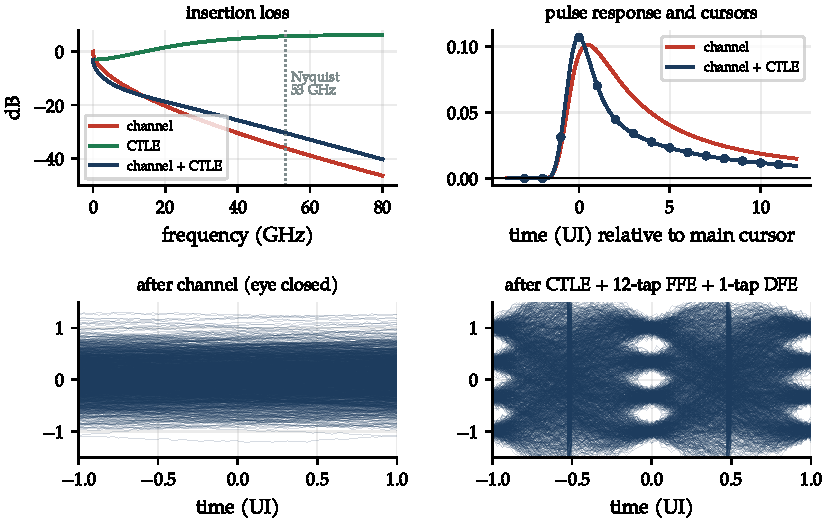
\includegraphics[width=0.92\linewidth]{figs/ch12_serdes}\caption{Equalizing a 212.5\,Gb/s PAM-4 lane (106.25\,GBd, synthetic channel with about
30\,dB loss at Nyquist). Top left: insertion loss of the channel, a CTLE with a zero near 13\,GHz, and their
cascade. Top right: single-UI pulse response before and after the CTLE, with the cursor samples marked
at one-UI spacing. Bottom: eye diagrams before equalization and after CTLE, a 12-tap symbol-spaced FFE
(zero-forcing, with three precursor taps) and a one-tap DFE. The DFE subtracts its correction for a whole
UI at a time, which produces the vertical discontinuities at the UI boundaries; only the centre of the eye,
where the slicer samples, matters.}\label{fig:ch12_serdes}\end{figure}

\subsection{The equalizer chain}

A SerDes uses the whole family of this chapter, split between analog and digital and between
transmitter and receiver:
\begin{itemize}
\item \textbf{Transmit FFE (de-emphasis).} A short FIR at the transmitter---typically a main
cursor with one to three precursor taps and one postcursor tap---pre-distorts the signal. Because the
transmitter has a peak-amplitude limit, pre-emphasis really \emph{de}-emphasises the low frequencies
rather than boosting the high ones. The receiver negotiates the tap values during link training.
\item \textbf{CTLE.} A \emph{continuous-time linear equalizer}, an analog high-pass stage with a
zero and two or more poles, provides 6--15\,dB of high-frequency peaking before the sampler. It is
cheap and reduces the load on everything after it, but it amplifies noise and crosstalk along with the
signal---linear equalization's usual price.
\item \textbf{Receive FFE.} In ADC-based receivers (the norm at 112\,Gb/s and above) a digital FFE of
tens of taps removes precursors and residual postcursors, as in Section~\ref{sec:ch12:fir}.
\item \textbf{DFE.} One to a dozen or more feedback taps cancel postcursor ISI without noise
enhancement. The first tap is the hard one: the decision on symbol $n-1$ must be made, multiplied and
subtracted before symbol $n$ is sliced, within one UI---9.4\,ps at 106\,GBd, less than the delay of a
few logic gates. Designers \term{loop-unroll} it (a \emph{speculative} DFE): compute the slicer
outputs for every possible value of the previous symbol in parallel and select the right one once that
symbol is known. For PAM-4 that is four speculative paths of three comparators each.
\item \textbf{Sequence detection.} Many 224\,Gb/s receiver designs add a short MLSE or reduced-state
detector after the FFE, replacing or supplementing the DFE, to gain back a few decibels.
\end{itemize}
Adaptation is almost always a variant of sign-sign LMS (for the analog and mixed-signal taps) or LMS
(in the DSP), running continuously in decision-directed mode after link training.

\begin{worked}[title=Why a DFE tap is worth more than an FFE tap]
In Figure~\ref{fig:ch12_serdes} the sampled pulse response after the CTLE has a precursor of 0.29
and a first postcursor of 0.66 relative to the main cursor, followed by a long tail. The 12-tap FFE
was designed to zero the precursors and the tail but to \emph{leave} a first postcursor of about 0.33
for the DFE. Removing it linearly would require the FFE to boost the frequencies where the channel is
weakest, raising the noise and crosstalk that the FFE passes through by several decibels. The DFE removes
it by subtracting a stored multiple of the previous decision, which contains no noise at all. The cost
is error propagation: an error in the previous PAM-4 symbol, typically to an adjacent level, leaves a
residual of $2b_1$ where $b_1$ is the tap weight---and if $b_1$ is a large fraction of the main
cursor, the next decision is likely to be wrong too. This is why PAM-4 Ethernet PHYs allow
\emph{precoding} (a $1/(1\oplus D)$ precoder modulo 4, introduced for 50\,Gb/s-per-lane PAM-4 and carried
forward): it converts a DFE error burst into, typically, just two symbol errors at its start and
end, which the Reed--Solomon FEC then handles.
\end{worked}

\begin{inpractice}[title=Reading a SerDes datasheet]
When you see a SerDes quoted as supporting ``40\,dB channels'', the loss is measured at the Nyquist
frequency, and the claim implies the whole chain above: typically a transmit FFE with several taps,
a CTLE with around 10\,dB or more of peaking, an ADC with six to eight bits of nominal resolution, a receive FFE of
tens of taps, and a DFE or MLSE, all adapted continuously. The receiver's target is not zero bit
errors but a raw BER better than the FEC threshold---around $2.4\times10^{-4}$ for the RS(544,514) ``KP4''
code used across 100--400\,Gb/s Ethernet. Power efficiency, in picojoules per bit, is the figure of
merit that decides which equalizer architecture wins; it is one of the most intensely optimised
numbers in the semiconductor industry.
\end{inpractice}

\section{Equalization in coherent optical receivers}
\label{sec:ch12:optical}

A coherent optical receiver (Chapter~\ref{ch:wireline}) mixes the incoming light with a local laser,
detects the in-phase and quadrature components of both polarizations, samples them at around two
samples per symbol, and hands the rest to DSP. Its equalizers are among the largest in any
communication system.

\subsection{Chromatic dispersion}

In single-mode fibre different wavelengths travel at different group velocities. At 1550\,nm standard
fibre has a dispersion parameter $D\approx17$\,ps/(nm\,km). A signal of symbol rate $R_s$ occupies a
wavelength range of about $\Delta\lambda\approx\lambda^2R_s/c$, so after a length $\ell$ its pulses
spread by $\Delta\tau\approx D\,\ell\,\Delta\lambda$, which in symbols is
\begin{equation}
N_{\mathrm{CD}}\approx\frac{D\,\ell\,\lambda^2R_s^2}{c}.
\label{eq:ch12:cd}
\end{equation}
Chromatic dispersion is a pure, lossless phase distortion, an all-pass filter
$H_{\mathrm{CD}}(\omega)=\exp(-j\beta_2\ell\omega^2/2)$ with $\beta_2=-D\lambda^2/(2\pi c)\approx-21.7$\,ps$^2$/km,
and it is \emph{static}: it changes only with the route. It is therefore compensated by a fixed
filter---the inverse all-pass---whose length grows linearly with distance and with the square of the
symbol rate (Figure~\ref{fig:ch12_cd}). Because thousands of taps are needed on long links, the
filter is always implemented in the frequency domain with overlap-save FFT processing, exactly the
complexity argument of Section~\ref{sec:ch12:fde}.

\mdcfig{ch12_cd}{Chromatic dispersion. Left: the power of a single 64\,GBd root-raised-cosine pulse
after 0, 5, 20 and 80\,km of standard single-mode fibre; after 80\,km it spans about 40 symbols. Right:
length of the CD-compensating FIR at two samples per symbol against distance, from~\eqref{eq:ch12:cd}.
Long-haul and transoceanic links need thousands to tens of thousands of taps.}

\begin{worked}[title=Sizing the CD equalizer of a 400ZR module]
The OIF 400ZR implementation agreement specifies dual-polarization 16-QAM at about 60\,GBd for
data-centre interconnect up to about 120\,km. Using~\eqref{eq:ch12:cd}:
$\Delta\lambda=\lambda^2R_s/c=(1.55\times10^{-6})^2(60\times10^9)/(3\times10^8)\approx0.48$\,nm; the
accumulated dispersion is $17\times120=2040$\,ps/nm, so $\Delta\tau\approx980$\,ps, or about 59 symbols.
At two samples per symbol the CD filter needs roughly 120 taps per polarization, plus margin for the
filter's own roll-off---easily done with a few-hundred-point FFT, in a pluggable module that must
dissipate only about 15--20\,W in total. A transpacific link of 10{,}000\,km at 130\,GBd would instead need
some tens of thousands of taps.
\end{worked}

\subsection{The butterfly equalizer}

After CD compensation, the two polarizations remain mixed. The fibre's birefringence rotates the
state of polarization randomly and continually (in aerial cables near railways or during lightning
strikes, at tens to hundreds of thousands of radians per second) and adds \emph{polarization-mode
dispersion} (PMD), a differential delay between two principal states. The receiver undoes this with a
$2\times2$ MIMO equalizer, the \term{butterfly equalizer} (Figure~\ref{fig:ch12_butterfly}):
\begin{equation}
\begin{aligned}
z_x[n]&=\vect w_{xx}^H\vect y_x[n]+\vect w_{xy}^H\vect y_y[n],\\
z_y[n]&=\vect w_{yx}^H\vect y_x[n]+\vect w_{yy}^H\vect y_y[n],
\end{aligned}
\end{equation}
four complex FIR filters of typically 10--30 taps at two samples per symbol. Their adaptation is blind:
in most commercial receivers it has been CMA (or its multi-modulus variants) for acquisition,
followed by decision-directed LMS, the same recipe as in Section~\ref{sec:ch12:blind} in its most
demanding setting, with the twist that CMA can converge with both outputs locked to the \emph{same}
polarization (the \emph{singularity} problem), which practical receivers prevent by initialisation
or by constraining $\vect w_{yx}, \vect w_{yy}$ to be orthogonal to $\vect w_{xx}, \vect w_{xy}$.
Chapter~\ref{ch:mimo} generalises the same idea to wireless MIMO.

\begin{figure}[htbp]\centering
\begin{tikzpicture}[>=Stealth, font=\small,
  blk/.style={draw=navy, fill=navy!6, thick, rounded corners=2pt, minimum height=0.7cm, minimum width=1.3cm, align=center},
  sum/.style={draw=navy, thick, circle, inner sep=0pt, minimum size=0.45cm},
  lbl/.style={font=\footnotesize}]
\node[lbl] (yx) at (0,1.2) {$y_x$};
\node[lbl] (yy) at (0,-1.2) {$y_y$};
\node[blk] (hxx) at (2.5,1.6) {$\vect w_{xx}$};
\node[blk] (hyx) at (2.5,0.5) {$\vect w_{yx}$};
\node[blk] (hxy) at (2.5,-0.5) {$\vect w_{xy}$};
\node[blk] (hyy) at (2.5,-1.6) {$\vect w_{yy}$};
\node[sum] (sx) at (4.6,1.2) {$+$};
\node[sum] (sy) at (4.6,-1.2) {$+$};
\draw[->] (yx) -- (1.0,1.2) |- (hxx.west); \draw[->] (1.0,1.2) |- (hyx.west);
\draw[->] (yy) -- (1.0,-1.2) |- (hyy.west); \draw[->] (1.0,-1.2) |- (hxy.west);
\draw[->] (hxx.east) -| (sx.north); \draw[->] (hxy.east) -- (sx.south west);
\draw[->] (hyx.east) -- (sy.north west); \draw[->] (hyy.east) -| (sy.south);
\node[blk, minimum width=2.4cm] (cpe) at (6.9,1.2) {carrier recovery,\\ slicer};
\node[blk, minimum width=2.4cm] (cpe2) at (6.9,-1.2) {carrier recovery,\\ slicer};
\draw[->] (sx) -- node[above,lbl]{$z_x$} (cpe.west); \draw[->] (sy) -- node[below,lbl]{$z_y$} (cpe2.west);
\node[lbl, text=accent, align=center] at (6.9,0) {CMA / DD-LMS\\ adapts all four filters};
\node[blk, fill=accent!8, draw=accent, minimum width=1.1cm, align=center] at (-1.8,0) {CD\\ comp.\\ (FFT)};
\draw[->, gray] (-1.2,0.2) -- (-0.3,1.1); \draw[->, gray] (-1.2,-0.2) -- (-0.3,-1.1);
\end{tikzpicture}
\caption{The $2\times2$ butterfly equalizer of a coherent optical receiver. After static
chromatic-dispersion compensation in the frequency domain, four adaptive FIR filters undo the
polarization rotation and PMD, each output drawing on both received polarizations.}
\label{fig:ch12_butterfly}
\end{figure}

\begin{inpractice}[title=The DSP of a coherent transceiver]
The receive DSP of a coherent optical module is a textbook of this chapter, in order: static CD
compensation in the frequency domain (Section~\ref{sec:ch12:fde}), timing recovery
(Chapter~\ref{ch:sync}), the adaptive $2\times2$ butterfly (this section), carrier frequency and phase
recovery, and soft-decision FEC decoding. Recent generations add nonlinear compensation and
transmit-side pre-emphasis for the analog bandwidth limits of the modulator and DAC. Running at
tens of gigabaud with parallelism of hundreds of samples per clock, the whole chain is one of the most
complex signal-processing ASICs made.
\end{inpractice}

\section{Echo cancellation: the same mathematics}
\label{sec:ch12:echo}

A two-wire telephone line carries both directions of a conversation on one pair; a \emph{hybrid}
transformer separates them at each end. Because the hybrid is balanced for a nominal line impedance
that never matches the real one exactly, some of the transmitted signal leaks into the local
receiver: \term{echo}. For a full-duplex modem the near-end echo can be much stronger than the
far-end signal, which has been attenuated by the whole line, so the echo must be suppressed by
perhaps 50--60\,dB or more. The solution is an \term{echo canceller}: an adaptive FIR filter driven by
the local transmit symbols that learns the echo path and subtracts a replica of the echo from the
received signal. The error signal is the received signal after cancellation, and the algorithm is
LMS.

Structurally this is the dual of an equalizer. An equalizer performs \emph{inverse modelling}: it
learns the inverse of the channel. An echo canceller performs \emph{system identification}: it learns
a model of the echo path itself. Both minimise a mean-square error with the same stochastic gradient,
and everything in Sections~\ref{sec:ch12:lms} and~\ref{sec:ch12:rls} applies---step size,
misadjustment, eigenvalue spread (now of the transmit signal, which is white for data and strongly
coloured for speech). The echo canceller has one pleasant difference: its input is the transmitter's
own clean symbol stream, so there are no decision errors to worry about.

Echo cancellation shaped modem history. V.32 (1984) was the first widely used standard to run
9600\,bit/s full duplex over a two-wire line by cancelling the echo instead of splitting the band; every
later voice-band modem, ISDN basic rate and HDSL did the same. Gigabit Ethernet (1000BASE-T) runs four
pairs in both directions simultaneously, so each receiver contains an echo canceller for its own pair
plus three near-end crosstalk (NEXT) cancellers for the other three---the same adaptive filter,
four times over. Telephone networks use \emph{network echo cancellers} (ITU-T G.168) with tails of
tens of milliseconds for the hybrid echo of long-distance calls, and every speakerphone, conferencing
system and smart speaker runs an \emph{acoustic} echo canceller with thousands of NLMS taps (usually in
the frequency domain, for the complexity reasons of Section~\ref{sec:ch12:fde}) to remove the
loudspeaker's sound from the microphone. The acoustic case adds a hard problem that data echo
cancellers do not face: \emph{double talk}, when the near-end talker speaks at the same time as the
far end, which must be detected so that adaptation is frozen before the near-end speech corrupts the
echo-path estimate.

\section{Neural-network equalizers}
\label{sec:ch12:nn}

Every equalizer in this chapter assumes a linear channel. Some channels are not: an optical fibre at
high launch power (the Kerr nonlinearity), a directly modulated laser, a power amplifier driven into
compression, a magnetic recording head. For these, researchers have revisited an old idea---nonlinear
adaptive equalizers, which date back to Volterra-series equalizers and to multilayer-perceptron
equalizers of the early 1990s---with modern machine learning. Convolutional and recurrent networks,
trained on known sequences exactly as an LMS equalizer is trained, can learn nonlinear distortions that
a linear FIR cannot, and in laboratory experiments on short-reach optical links with strong
nonlinearity they have shown gains of a decibel or more over linear equalizers.

The engineering reality check is complexity. A neural equalizer that needs thousands of
multiplications per symbol competes with a Volterra or linear equalizer that needs tens, in hardware
where power per bit is the figure of merit. The fair comparison is always at \emph{equal complexity},
and on linear channels a well-designed classical equalizer is already optimal---a neural network can at
best learn to imitate it. The most promising uses are where the channel is genuinely nonlinear or poorly
modelled, and where the network can be kept small or its structure borrowed from the physics (for
instance, networks that unfold the split-step Fourier method used to model fibre propagation).
Equalization is, after all, where adaptive learning systems began: LMS was invented to train a neuron.

\section{Summary}
\label{sec:ch12:summary}

\begin{keyidea}[title=Equalization in ten lines]
\begin{itemize}
\item After the (whitened) matched filter, every linear ISI channel is an FIR filter in white noise;
the matched-filter bound $E_s\|h\|^2/N_0$ is the benchmark.
\item Linear ZF inverts the channel and pays the harmonic mean of $|H|^{-2}$ in noise: fatal at nulls.
\item Linear MMSE regularises the inverse with $N_0/E_s$; remove its bias, and use
$\mathrm{SNR}_U=\mathrm{SNR}-1$.
\item Finite equalizers need a sensible length (a few channel spans) and delay; fractional spacing
removes sensitivity to sampling phase.
\item LMS is cheap and robust but slows down with eigenvalue spread; RLS converges in $\approx2L$ steps
at $\mathcal O(L^2)$ cost.
\item CMA equalizes blindly using the constellation's constant modulus, leaving a phase ambiguity.
\item The DFE cancels postcursors with past decisions: geometric-mean performance, preserves mutual
information, but propagates errors. THP moves it to the transmitter.
\item MLSE (Viterbi on the ISI trellis) is optimal and often reaches the MFB, at exponential cost;
RSSE/DFSE and minimum-phase prefilters make it practical.
\item For long channels, FFT-based equalization (SC-FDE, OFDM) wins on complexity; turbo equalization
lets the code help the equalizer.
\item The same mathematics runs 224G SerDes, coherent optics and echo cancellers.
\end{itemize}
\end{keyidea}

\problems
\begin{enumerate}[label=\thechapter.\arabic*]
\item \emph{(Noise enhancement.)} For the channel $H(z)=1+az^{-1}$ with $|a|<1$ and white noise of
variance $N_0$, show that the infinite-length ZF equalizer's output noise variance is
$N_0/(1-|a|^2)$. What happens for $|a|>1$, and what equalizer would you use instead?

\item \emph{(MMSE and bias.)} For the same channel, derive the infinite-length MMSE equalizer and its
MSE, and verify numerically that $\mathrm{SNR}_{\mathrm{MMSE}}=1/J_{\min}$ exceeds the unbiased SNR by
exactly one (in linear units). For $a=0.9$ and $E_s/N_0=10$\,dB, what is the bias factor $\beta$?

\item \emph{(Three means.)} Prove that for any non-negative $S(\theta)$ the harmonic, geometric and
arithmetic means satisfy $\mathrm{HM}\le\mathrm{GM}\le\mathrm{AM}$, and interpret each inequality as
a statement about linear ZF, ZF-DFE and the matched-filter bound.

\item \emph{(Minimum phase.)} Find the minimum-phase and maximum-phase channels with the same magnitude
response as $h=[1,\ -2.5,\ 1]$. Which one gives the better ZF-DFE, and by how many decibels relative to
using $h$ directly without a precursor-cancelling feedforward filter?

\item \emph{(Delay selection.)} Show that the MSE of an MMSE FIR equalizer for all delays can be read
off the diagonal of $\vect I-\vect G^H(\vect G\vect G^H+\sigma^2\vect I)^{-1}\vect G$. Use this to find the
best delay for channel C with $L=21$ at 20\,dB.

\item \emph{(LMS step size.)} An LMS equalizer has 31 taps and input power 0.5. Find the step size for
a misadjustment of 10\%. If the channel's eigenvalue spread is 50 and the largest eigenvalue is 2,
estimate the time constant of the slowest mode.

\item \emph{(NLMS.)} Show that NLMS with $\tilde\mu=1$ solves the problem
$\min\|\vect w_{n+1}-\vect w_n\|^2$ subject to $d_n=\vect w_{n+1}^H\vect y_n$.

\item \emph{(RLS derivation.)} Derive the RLS recursion~\eqref{eq:ch12:rls} from the cost
\eqref{eq:ch12:rlscost} using the matrix inversion lemma, and count the multiplications per update for
$L$ taps.

\item \emph{(CMA constant.)} Compute $R_2$ for unit-energy QPSK, 16-QAM and 64-QAM. Show that for QPSK
the CM cost of a perfectly equalized output is zero, while for 16-QAM it is not, and compute its value.

\item \emph{(THP power.)} Show that the THP output for $M$-PAM is uniform on $[-M,M)$ when the
channel's feedback is sufficiently ``mixing'', and derive the precoding loss
\[
  10\log_{10}\frac{M^2}{M^2-1}\ \text{dB}.
\]
Evaluate it for $M=2,4,16$.

\item \emph{(MLSE distance.)} For BPSK over $h=[1,\ 1]/\sqrt2$ (the duobinary channel) find
$d^2_{\min}$ and the MLSE loss relative to the MFB. Compare with the loss of the ZF-DFE.

\item \emph{(Complexity.)} A single-carrier link at 50\,Msymbol/s faces a 4\,\textmu s delay spread.
Compare the complex multiplies per second of (a) a time-domain FFE of three channel spans, and (b) an
SC-FDE with $N=1024$ and a prefix covering the delay spread. What is the prefix overhead?

\item \emph{(Chromatic dispersion.)} Using~\eqref{eq:ch12:cd}, compute the CD memory in symbols of
a 130\,GBd signal over 80\,km and over 6000\,km of standard fibre. How many FFT points would you use for
overlap-save compensation of the 6000\,km case, and why?

\item \emph{(Simulation.)} Using \texttt{commlib.eqadv.mmse\_dfe\_fir} and \texttt{dfe\_run}, reproduce
the DFE curves of Figure~\ref{fig:ch12_dfe_ber} and measure the distribution of error-burst lengths at
$E_b/N_0=8$\,dB. How does it change if you increase $L_b$ from 2 to 6?

\item \emph{(Simulation.)} Extend \texttt{lab06\_equalization.py}: implement a $T/2$ fractionally spaced
LMS equalizer on an RRC-shaped signal, sweep the sampling phase, and reproduce the behaviour of
Figure~\ref{fig:ch12_fse}. Then add tap leakage and show that it prevents tap wandering in a long run
with fixed-point (16-bit) coefficients.
\end{enumerate}

\furtherreading
\begin{itemize}
\item J.~G.~Proakis and M.~Salehi, \emph{Digital Communications}, 5th ed., McGraw-Hill, 2008. Chapters 9
and 10 are the classical treatment of ISI channels and equalization, and the source of the benchmark
channels used in this chapter.
\item J.~R.~Barry, E.~A.~Lee and D.~G.~Messerschmitt, \emph{Digital Communication}, 3rd ed., Kluwer,
2004. The most careful textbook derivation of the WMF, the DFE and MLSE, with the spectral-factorization
view used here.
\item S.~Haykin, \emph{Adaptive Filter Theory}, 5th ed., Pearson, 2014; and A.~H.~Sayed,
\emph{Adaptive Filters}, Wiley, 2008. The two standard references for LMS, RLS and their relatives, with
the equalizer experiments reproduced in Figure~\ref{fig:ch12_lms_rls}.
\item S.~U.~H.~Qureshi, ``Adaptive equalization,'' \emph{Proc.\ IEEE}, 73(9), 1985. A classic tutorial
written when adaptive equalizers were the heart of every modem; still the best short introduction.
\item G.~D.~Forney, Jr., ``Maximum-likelihood sequence estimation of digital sequences in the presence of
intersymbol interference,'' \emph{IEEE Trans.\ Inf.\ Theory}, 18(3), 1972. The paper that introduced the
WMF and Viterbi equalization.
\item J.~M.~Cioffi, G.~P.~Dudevoir, M.~V.~Eyuboglu and G.~D.~Forney, Jr., ``MMSE decision-feedback
equalizers and coding,'' Parts I and II, \emph{IEEE Trans.\ Commun.}, 43(10), 1995. The
mutual-information interpretation of the unbiased MMSE-DFE.
\item C.~R.~Johnson, Jr.\ et al., ``Blind equalization using the constant modulus criterion: a review,''
\emph{Proc.\ IEEE}, 86(10), 1998. Theory and practice of CMA.
\item R.~F.~H.~Fischer, \emph{Precoding and Signal Shaping for Digital Transmission}, Wiley, 2002. THP and its
relatives in depth, including DSL applications.
\item R.~Koetter, A.~C.~Singer and M.~T\"uchler, ``Turbo equalization,'' \emph{IEEE Signal Processing
Magazine}, 21(1), 2004. An accessible tutorial with the soft-interference-cancellation equalizer.
\item D.~Falconer, S.~L.~Ariyavisitakul, A.~Benyamin-Seeyar and B.~Eidson, ``Frequency domain equalization
for single-carrier broadband wireless systems,'' \emph{IEEE Commun.\ Mag.}, 40(4), 2002.
\item S.~J.~Savory, ``Digital coherent optical receivers: algorithms and subsystems,'' \emph{IEEE J.\ Sel.\
Topics Quantum Electron.}, 16(5), 2010. The standard reference for CD compensation and the butterfly
equalizer.
\item R.~W.~Lucky, ``Automatic equalization for digital communication,'' \emph{Bell Syst.\ Tech.\ J.},
44(4), 1965; and B.~Widrow and S.~D.~Stearns, \emph{Adaptive Signal Processing}, Prentice Hall, 1985. Where
it all began.
\end{itemize}
